%% This is an example first chapter.  You should put chapter/appendix that you
%% write into a separate file, and add a line \include{yourfilename} to
%% main.tex, where `yourfilename.tex' is the name of the chapter/appendix file.
%% You can process specific files by typing their names in at the 
%% \files=
%% prompt when you run the file main.tex through LaTeX.
\chapter{Use Case 1 - Both Drug and Target Side} \label{Use Case}

\emph{Use case} ini melibatkan kedua sisi yaitu \emph{Drug-side} dan \emph{Target-side}. pada \emph{use case} ini, input dari kedua sisi harus ada.

\section{Plant-Disease}

Pada contoh ini, input dari \emph{drug-side} berupa tanaman (Plant) dan input dari \emph{target-side} berupa penyakit (Disease). Contoh ini mencari apakah dari tanaman yang diinputkan memiliki khasiat terhadap penyakit yang diinputkan, dan jika \textbf{ya}, maka apa saja senyawa dalam tanaman itu dan protein dalam penyakit itu yang ikut berperan.

\begin{figure}[H]
	\centering
	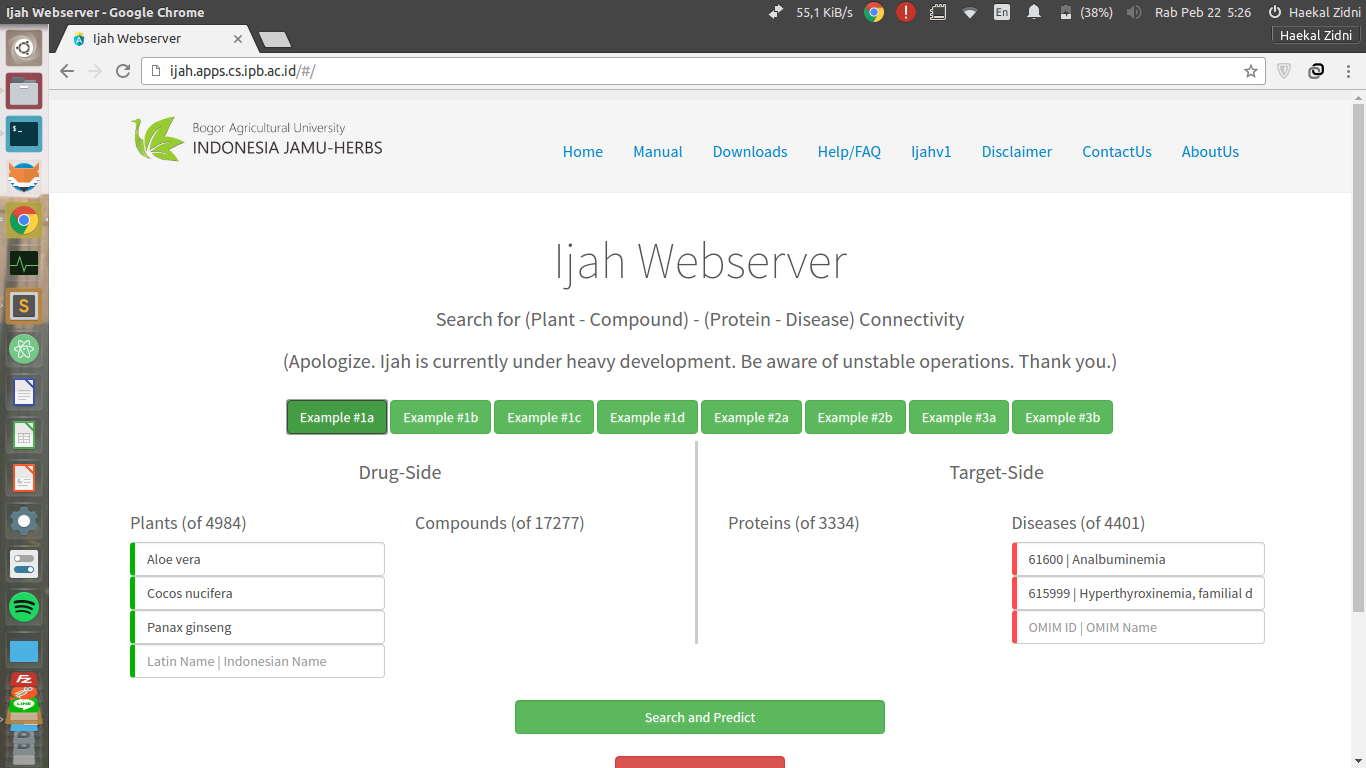
\includegraphics[scale=0.3]{example_1a.png}
	\caption{Contoh \emph{use case} input Plant dan Disease}
	\label{fig:example_1a}
\end{figure}

\subsection{Input}
Ijah Webserver memiliki fitur \emph{autocomplete} pada form input, ketika hasil \emph{autocomplete} sudah menunjukkan obyek yang diinginkan, klik nama obyek tersebut.

\begin{figure}[H]
	\centering
	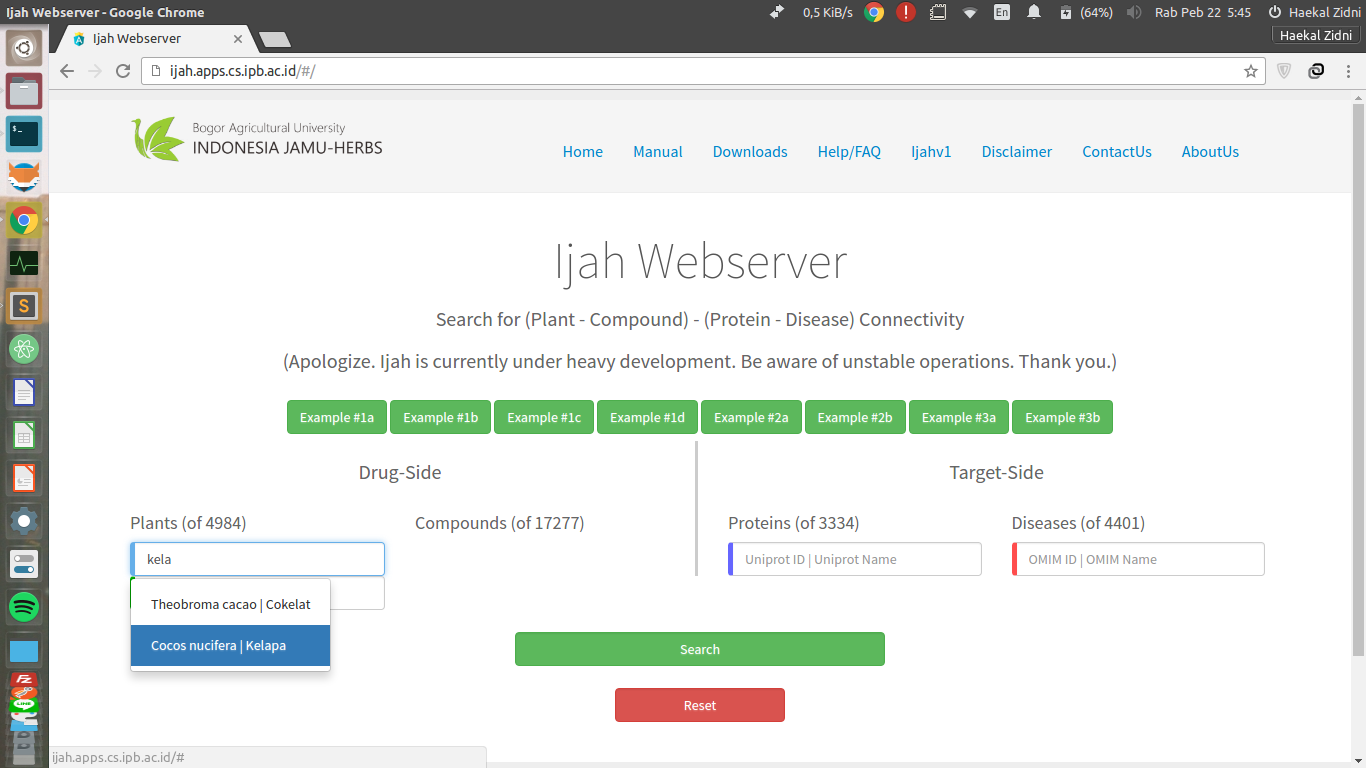
\includegraphics[scale=0.3]{ijah_autocomplete_click.png}
	\caption{Sorot dan klik hasil yang dimaksud untuk memasukkannya pada input}
	\label{fig:ijah_autocomplete_click}
\end{figure}

\begin{figure}[H]
	\centering
	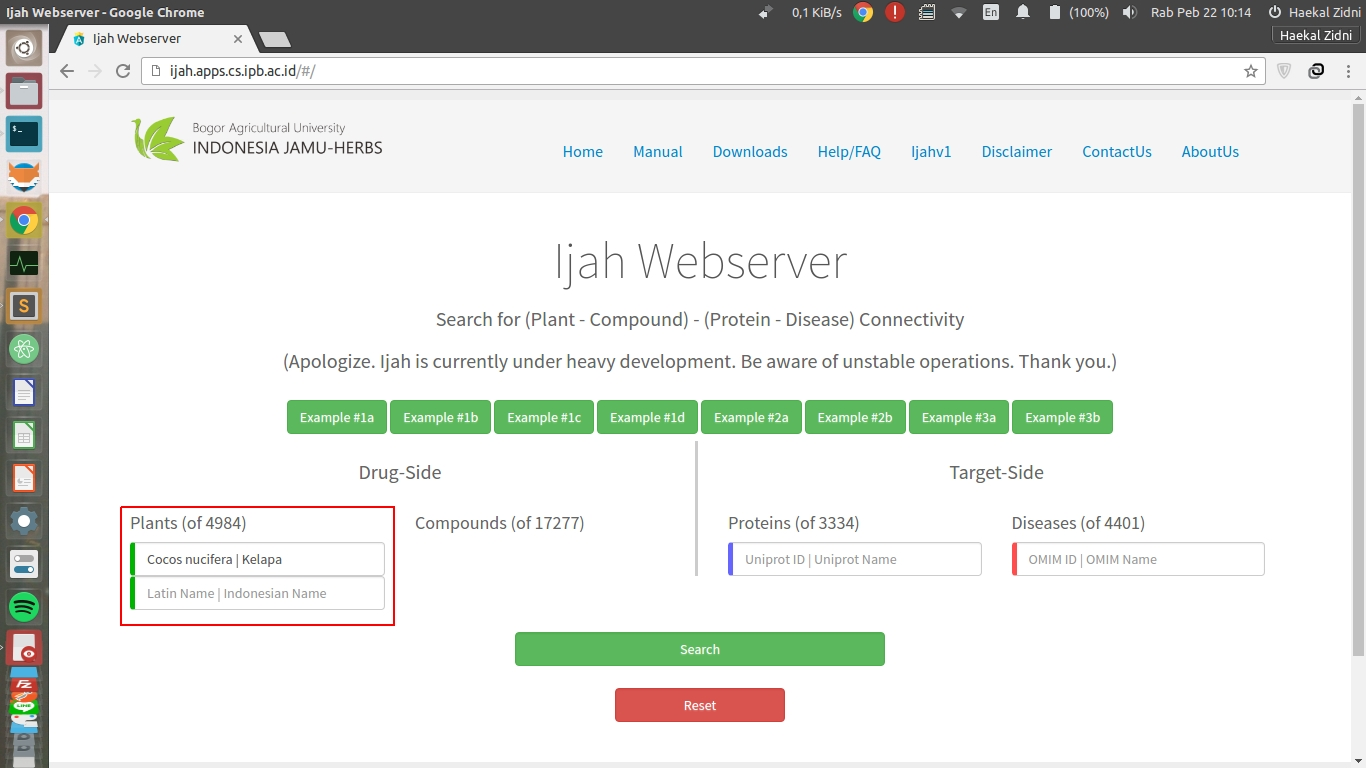
\includegraphics[scale=0.3]{ijah_autocomplete_complete.png}
	\caption{Setelah diklik input akan terlengkapi}
	\label{fig:ijah_autocomplete_complete}
\end{figure}

Pada jenis \emph{use case} ini (kedua sisi \emph{drug-side} dan \emph{target-side} terisi) perhatikan kembali Gambar 2.1\label{fig:example_1a}, tombol untuk melanjutkan pencarian memiliki label \textbf{Search and Predict}. Ini akan berbeda dengan kedua use case selanjutnya (yang hanya melibatkan satu \emph{side}) yang hanya akan berlabelkan \textbf{Search}.

Jika ingin mengosongkan input kembali, anda dapat mengklik tombol \textbf{Reset} di bawah tombol Search and Predict. Jika input sudah sesuai keinginan, lanjutkan dengan mengklik \textbf{Search and Predict}.

\subsection{Output}
Dengan contoh \emph{use case} seperti pada Gambar 2.1\label{fig:example_1a}, setelah menekan \textbf{Search and Predict} maka hasil output akan muncul. Ada tiga jenis output yaitu 

\begin{itemize}
\item \emph{Connectivity Graph Output}
\item \emph{Connectivity Text Output}
\item \emph{Metadata Text Output}
\end{itemize}

Hasil \emph{Connectivity Graph Output} untuk contoh diatas (3 input tanaman dan 2 input penyakit) adalah sebagai berikut

\begin{figure}[H]
	\centering
	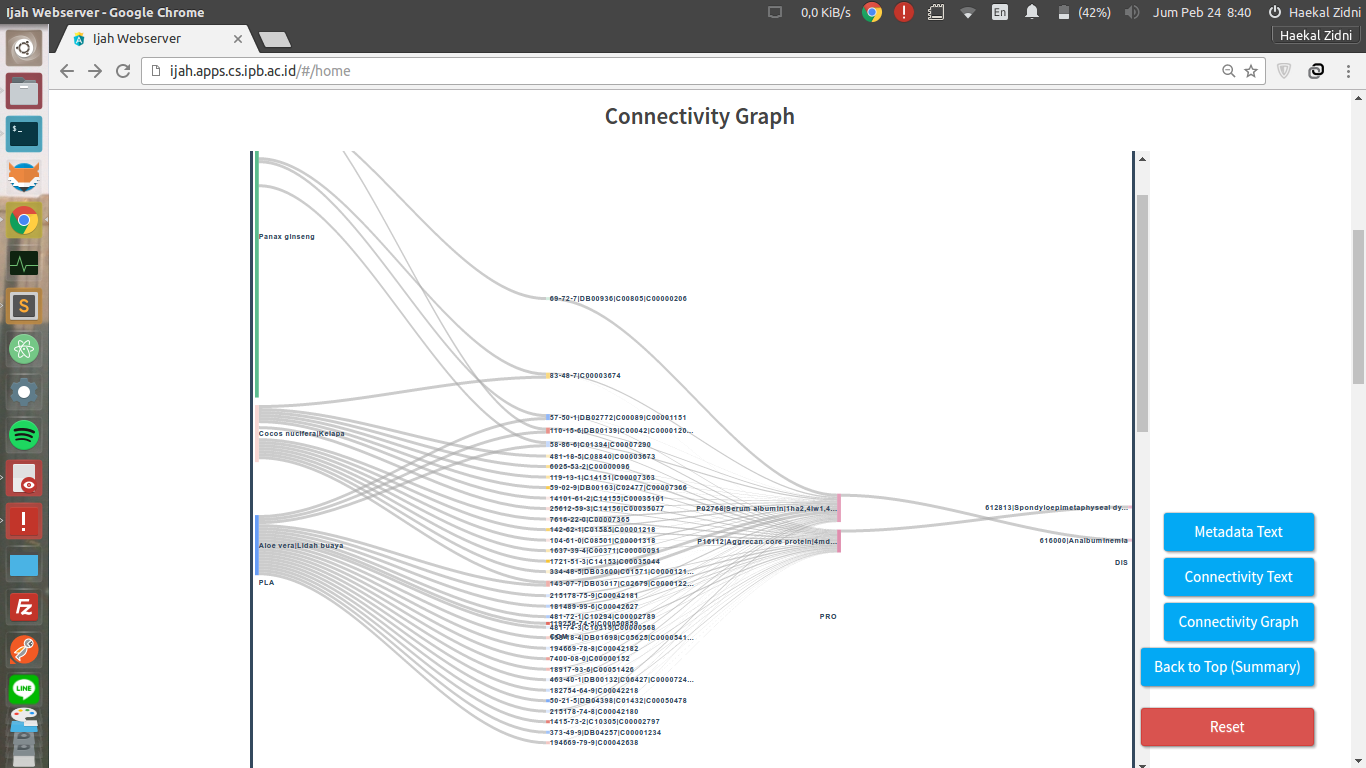
\includegraphics[scale=0.3]{ijah_example_1a_output.png}
	\caption{Connectivity Graph Output pada use case Predict Plant-Disease}
	\label{fig:ijah_example_1a_output}
\end{figure}

\textbf{Catatan:} jika graf terus di-scroll sampai habis maka akan ada tombol \textbf{Download} untuk mengunduh gambar graf tersebut.

Terlihat ada koneksi dari tanaman dan penyakit yang diinputkan. Dapat dilihat senyawa apa yang terkandung dalam tanaman tersebut dan mana yang memiliki hubungan kepada protein yang ada pada penyakit yang diinputkan.

Hasil \emph{Connectivity Text Output} untuk contoh diatas

\begin{figure}[H]
	\centering
	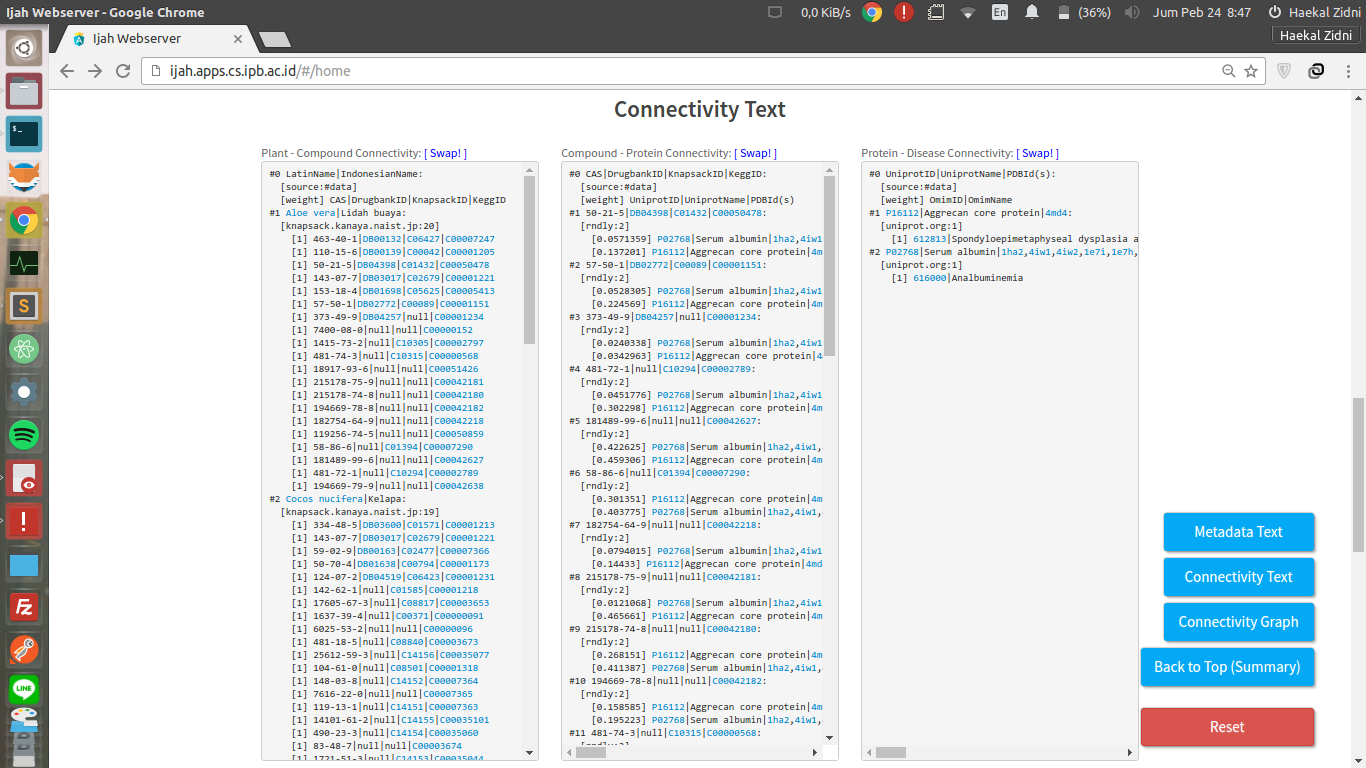
\includegraphics[scale=0.3]{ijah_example_1a_text.png}
	\caption{Connectivity Text Output pada use case Predict Plant-Disease}
	\label{fig:ijah_example_1a_text}
\end{figure}

Pada \emph{connectivity text output} ini bisa dilihat sumber data, serta skor konektivitas antar item, dan ID item yang merujuk pada sumber datanya (DrugBank, KnapSack, Uniprot, OMIM, dsb). Data teks dapat di-\emph{swap} misal dari Plant-Compound menjadi Compound-Plant dengan mengklik \textbf{Swap!} pada bagian atas tiap kotak teks. Pada bagian bawah kotak teks tersedia tombol untuk mengunduh file teks \emph{connectivity text output}.

\begin{figure}[H]
	\centering
	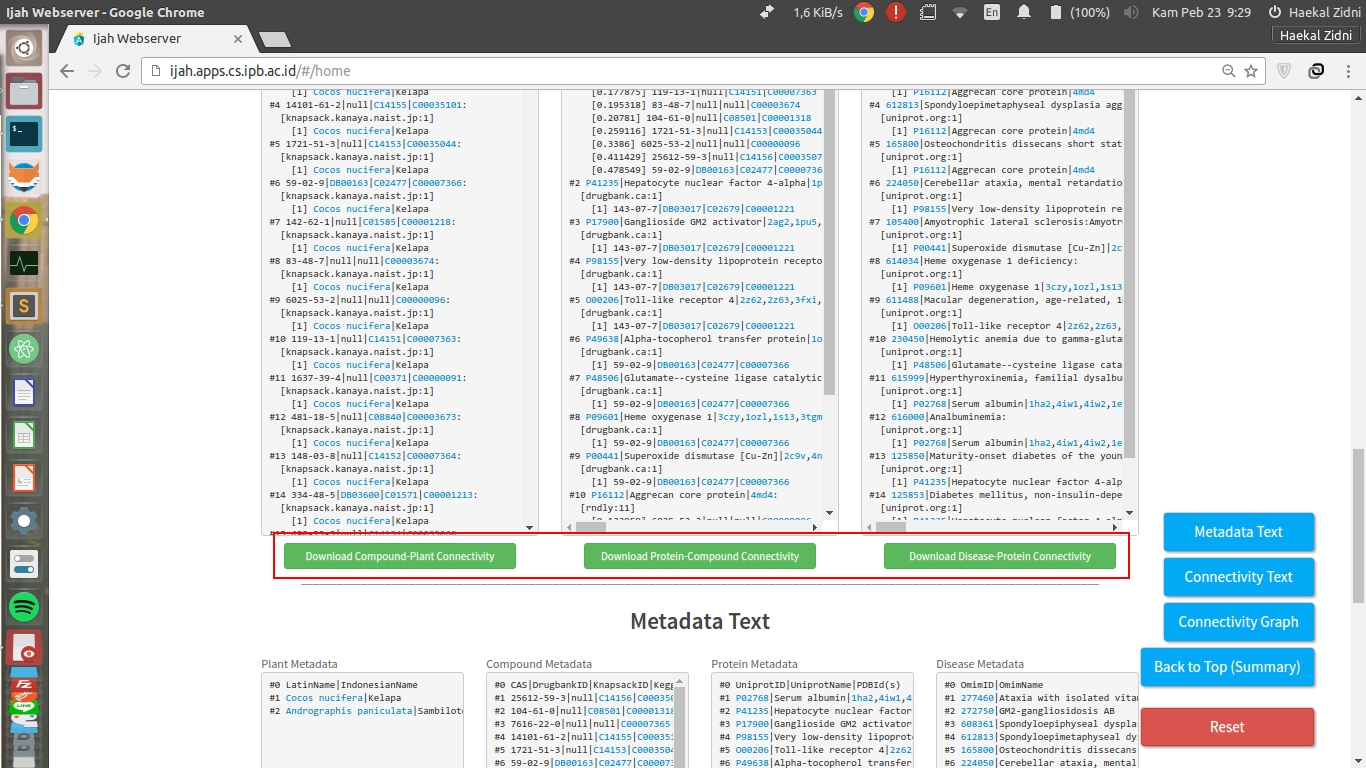
\includegraphics[scale=0.3]{ijah_text_download.png}
	\caption{Tombol Download untuk mengunduh file \emph{Connectivity Text Output}}
	\label{fig:ijah_text_download}
\end{figure}.

Hasil \emph{Metadata Text Output} untuk contoh diatas

\begin{figure}[H]
	\centering
	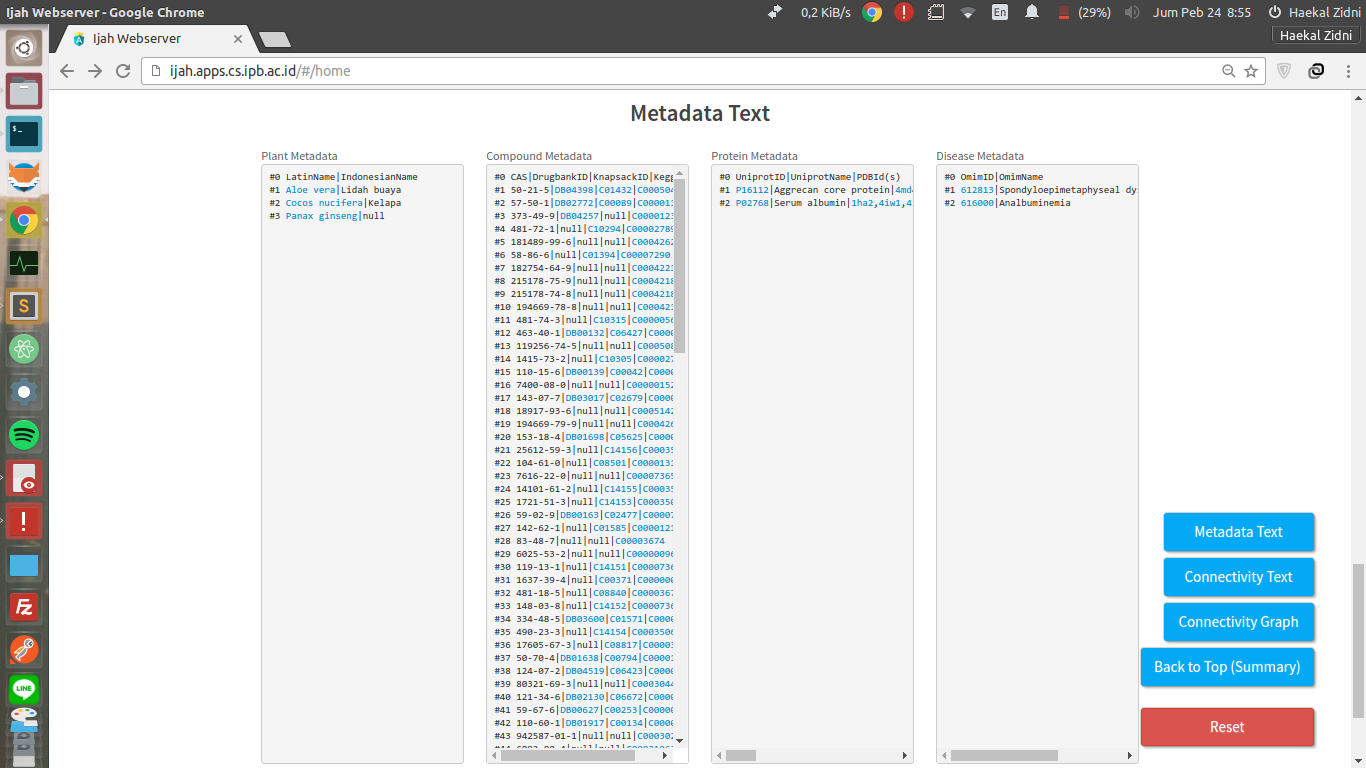
\includegraphics[scale=0.3]{ijah_example_1a_meta.png}
	\caption{Metadata Text Output pada use case Predict Plant-Disease}
	\label{fig:ijah_example_1a_meta}
\end{figure}

\emph{Metadata text output} memiliki tampilan yang mirip dengan \emph{connectivity text output} namun memiliki isi yang berbeda. Jika \emph{connectivity text output} berisikan konektivitas antar item (plant-compound, compound-protein, protein-disease) maka pada \emph{metadata text output} hanya berisi metadata dari setiap item yang terlibat (metadata dari setiap plant, compound, protein, dan disease yang ada). Metadata tidak bisa di-\emph{swap} sebagaimana connectivity text namun tetap bisa diunduh melalui tombol \textbf{Download} yang berada di bawah kotak teks.

\section{Plant-Protein}
Contoh lain dari \emph{use case} Both Drug-side and Target-side adalah Plant-Protein, dimana input berupa tanaman (Plant) dan Protein, yaitu apakah tanaman yang diinput memiliki kaitan dengan protein yang dinputkan. Perbedaan pada contoh Plant-Disease hanya pada input, selebihnya outputnya sama.

\section{Compound-Protein}
Pada contoh Compound-Protein input berupa senyawa (Compound) dan Protein, yaitu mencari apakah suatu senyawa input terkait dengan protein yang diinputkan. Perbedaan pada contoh Plant-Disease hanya pada input, selebihnya outputnya sama.

\section{Compound-Disease}
Pada contoh Compound-Disease input berupa senyawa (Compound) dan penyakit (Disease), yaitu mencari apakah senyawa input terkait dengan penyakit yang diinputkan. Perbedaan pada contoh Plant-Disease hanya pada input, selebihnya outputnya sama.

\section{Tambahan: \emph{Jumping} Pada Output}
Ada cara mudah untuk menuju satu jenis output secara spesifik, yaitu dengan \textbf{Jump}. Menu Jump ada pada bagian awal setelah Summary atau di bagian kanan bawah layar.

\begin{figure}[H]
	\centering
	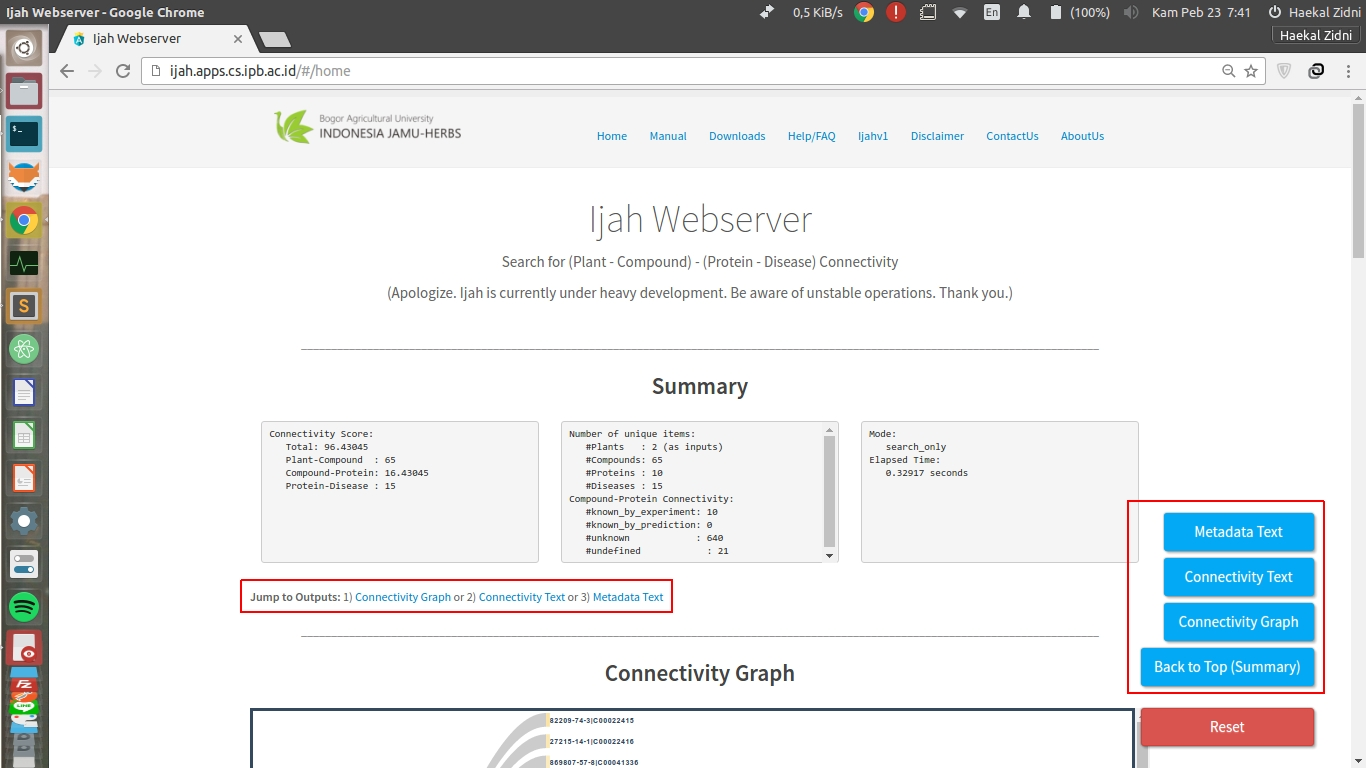
\includegraphics[scale=0.3]{ijah_output_jump.png}
	\caption{Output Jump Menu pada Ijah Webserver}
	\label{fig:ijah_output_jump}
\end{figure}

Jika tombol jump terasa menghalangi layar (terjadi pada layar dengan resolusi kurang dari 1920x1080) maka dapat diatasi dengan mengatur zoom browser menjadi 75\%

\begin{figure}[H]
	\centering
	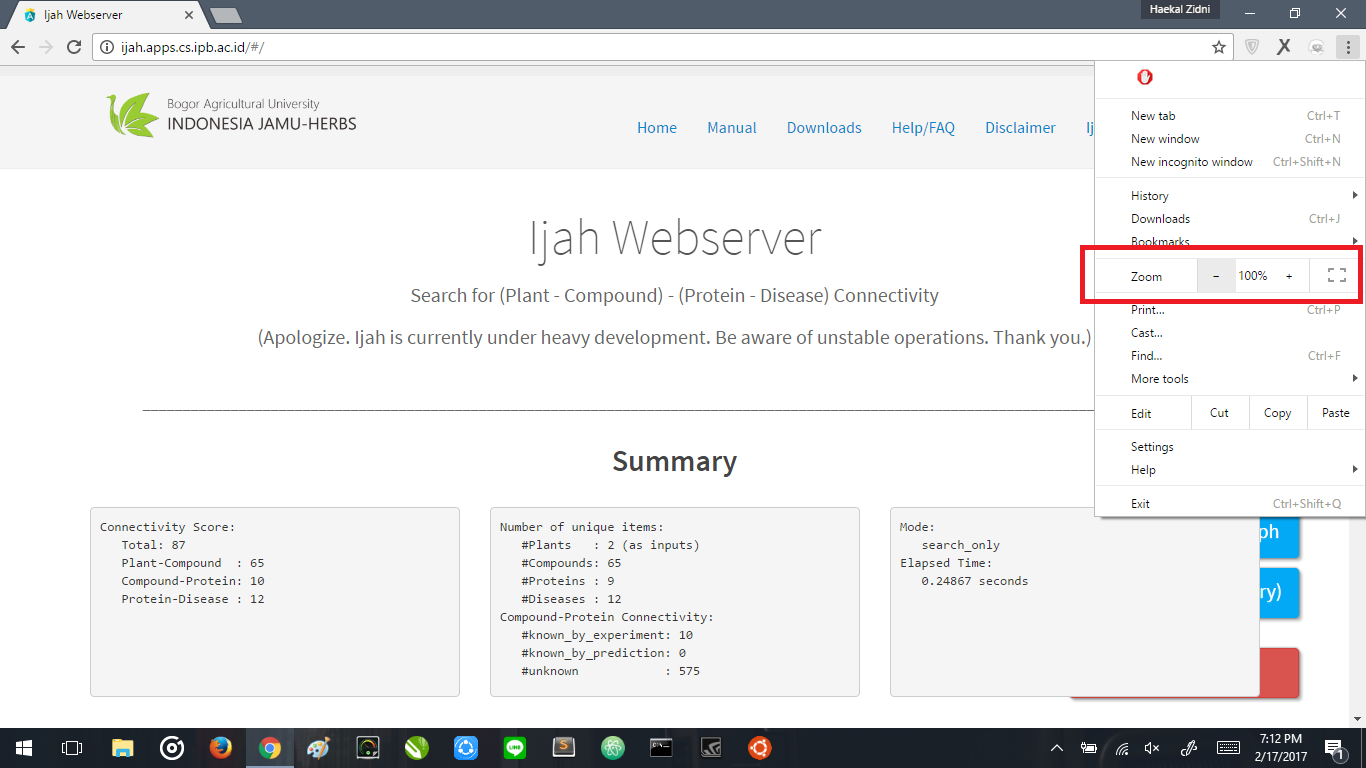
\includegraphics[scale=0.4]{chrome_zoom.png}
	\caption{Menu Zoom pada Chrome}
	\label{fig:chrome_zoom}
\end{figure}

Lakukan Zoom Out hingga 75\% dengan mengklik tombol \textbf{minus [-]}

\begin{figure}[H]
	\centering
	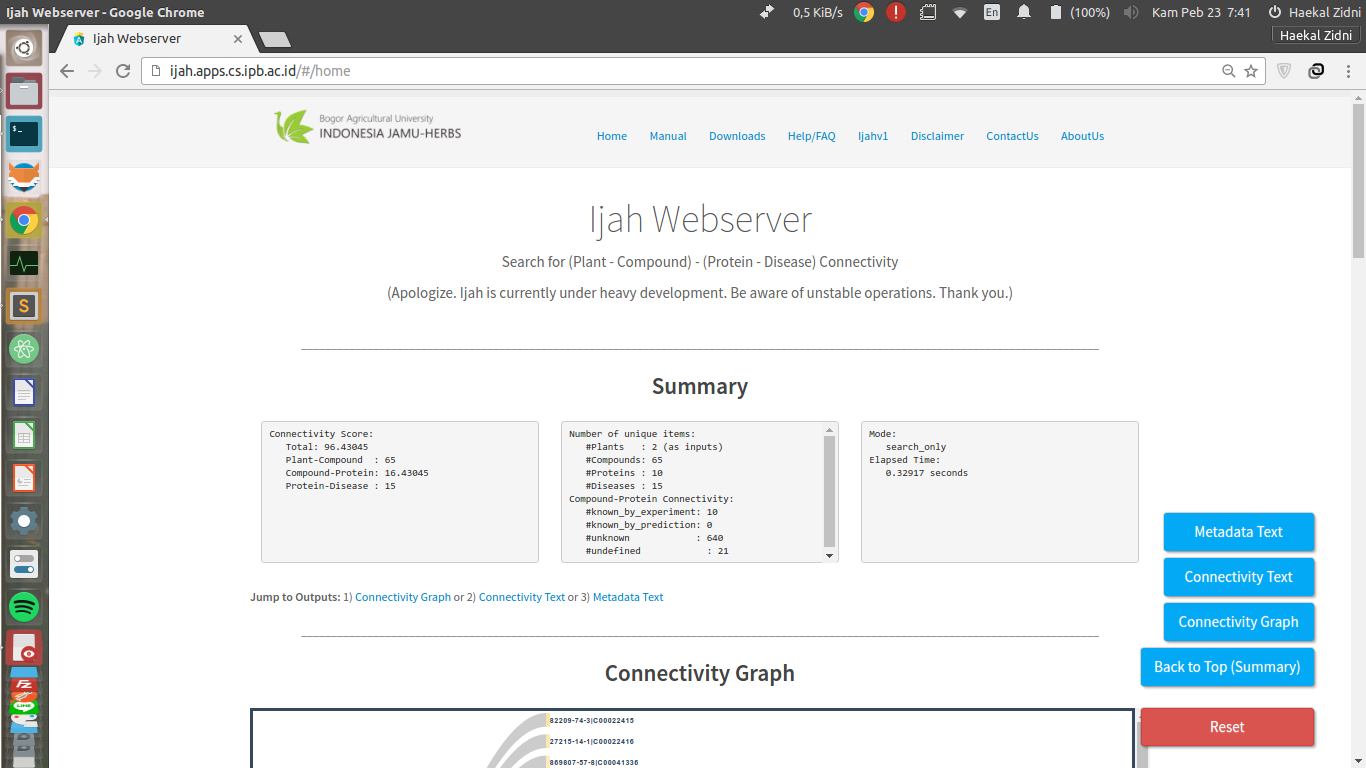
\includegraphics[scale=0.3]{ijah_zoom75.png}
	\caption{Hasil zoom ke 75\%}
	\label{fig:ijah_zoom75}
\end{figure}

Untuk melakukan Zoom Out dapat juga dilakukan menggunakan keyboard shortcut dengan menekan \textbf{Ctrl} + \textbf{-} secara bersamaan hingga 75\%.

% \subsection{Examples}

% \begin{figure}[H]
% 	\centering
% 	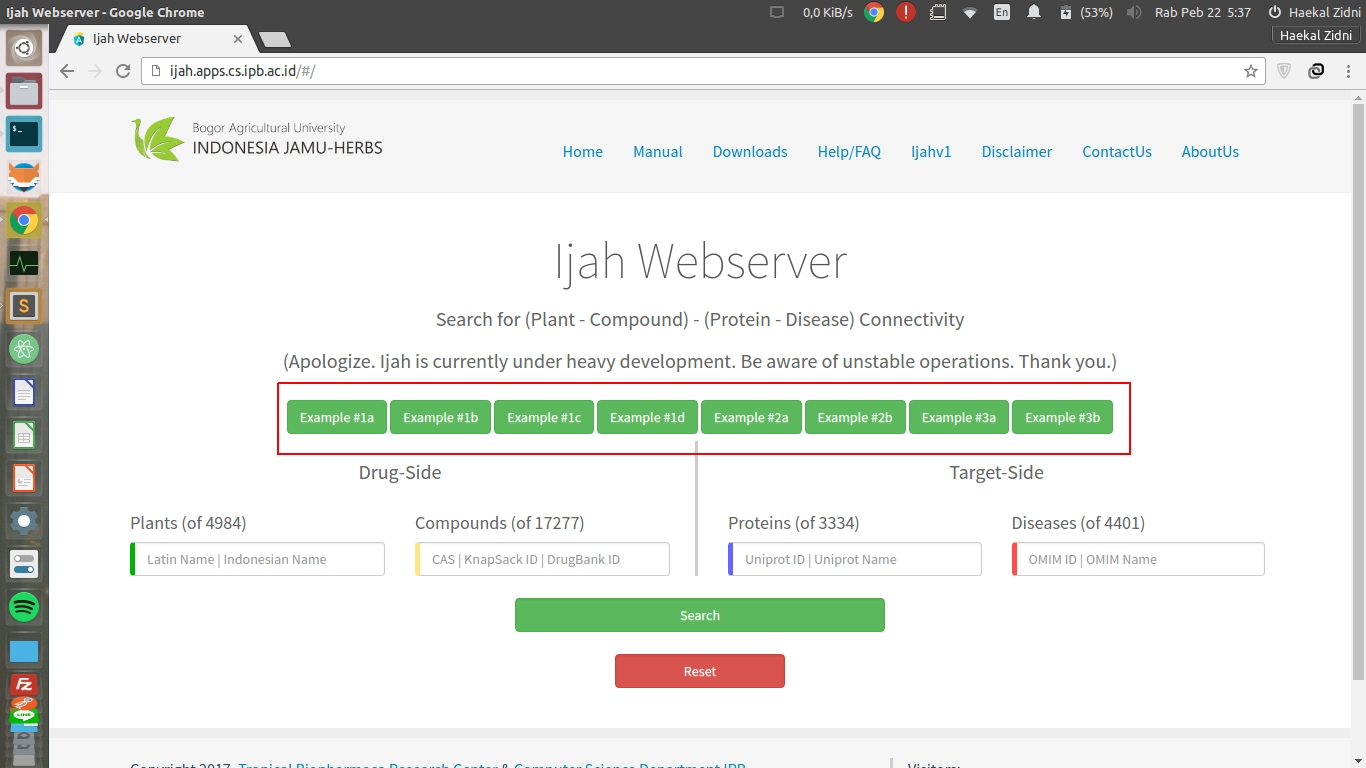
\includegraphics[scale=0.3]{ijah_examples.png}
% 	\caption{Deretan tombol \emph{Examples}}
% 	\label{fig:ijah_examples}
% \end{figure}

% Deretan tombol Examples merupakan contoh-contoh Use Case dalam penggunaan Ijah Webserver. Dimana Example 1 a\-d merupakan contoh end\-to\-end dari sisi Drug Side dan Target side, sedangkan Example  2 a\-b merupakan contoh pencarian pada Drug Side saja, dan Example 3 a\-b  merupakan contoh pencarian pada Target Side saja

% \begin{enumerate} [topsep=0mm]
% \itemsep0mm

% \item \textbf{Example 1a}
% \begin{figure}[H]
% 	\centering
% 	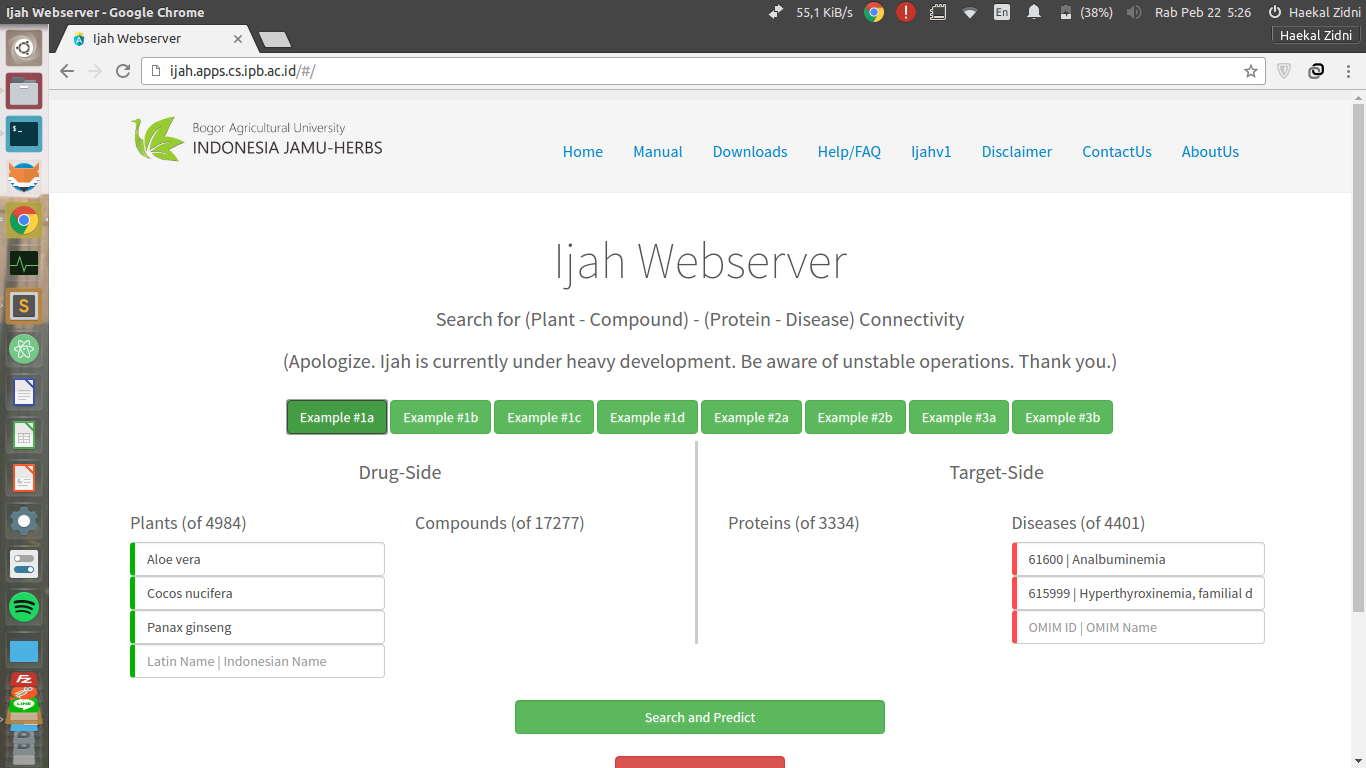
\includegraphics[scale=0.3]{example_1a.png}
% 	\caption{Example 1a}
% 	\label{fig:example_1a}
% \end{figure}

% Example 1a merupakan contoh use\-case pencarian antara Plants di sisi Drug\-side dan Diseases pada Target\-side, merepresentasikan pencarian “Apakah tanaman\-tanaman yang diinputkan memiliki hubungan dengan penyakit\-penyakit yang diinputkan”. Hasil yang ditunjukkan adalah hubungan antara tanaman pada input dan penyakit pada input, termasuk senyawa dan protein yang terkait.

% \item \textbf{Example 1b}
% \begin{figure}[H]
% 	\centering
% 	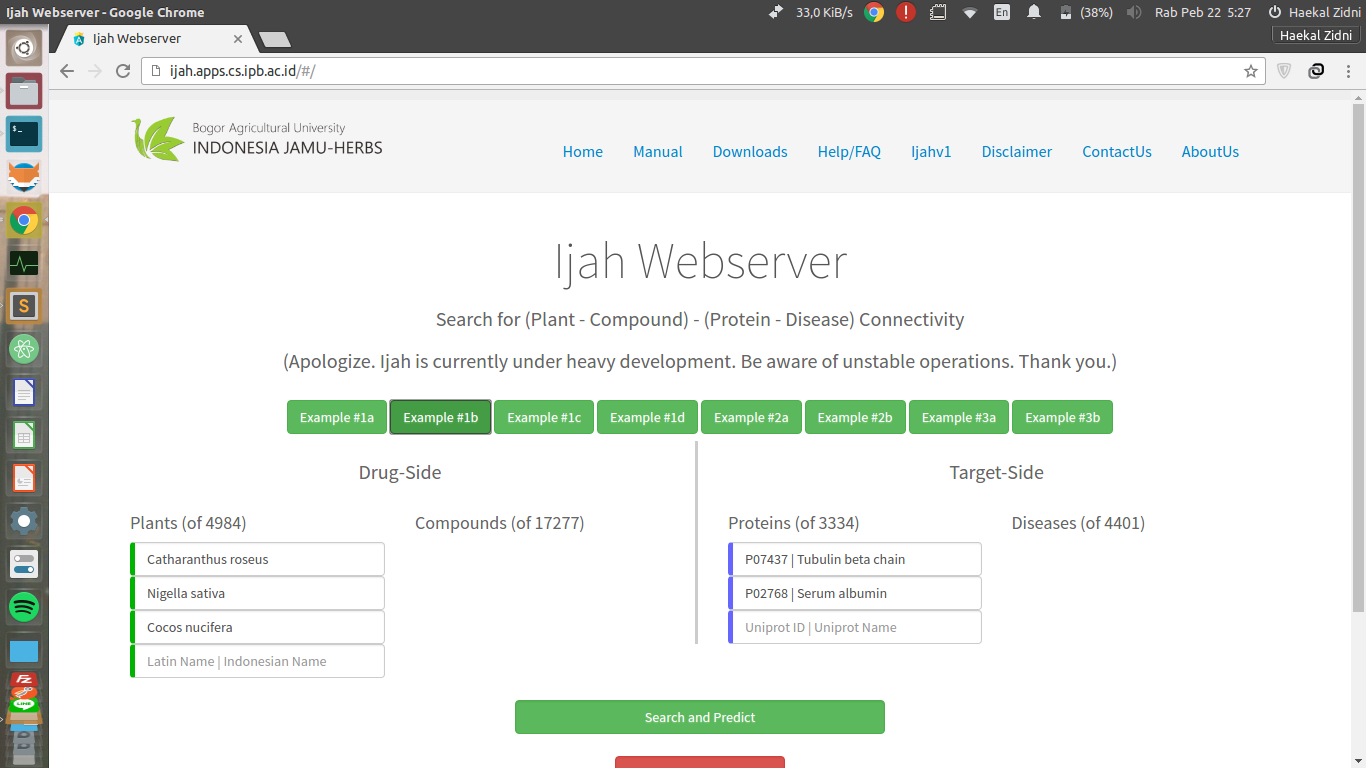
\includegraphics[scale=0.3]{example_1b.png}
% 	\caption{Example 1b}
% 	\label{fig:example_1b}
% \end{figure}

% Example 1b merupakan contoh use\-case pencarian antara Plants di sisi Drug\-side dan Proteins pada Target\-side, merepresentasikan pencarian “Apakah tanaman\-tanaman yang diinputkan memiliki hubungan dengan protein\-protein yang diinputkan”. Hasil yang ditunjukkan adalah hubungan antara tanaman pada input dan protein pada input, termasuk senyawa dan penyakit yang terkait.

% \item \textbf{Example 1c}
% \begin{figure}[H]
% 	\centering
% 	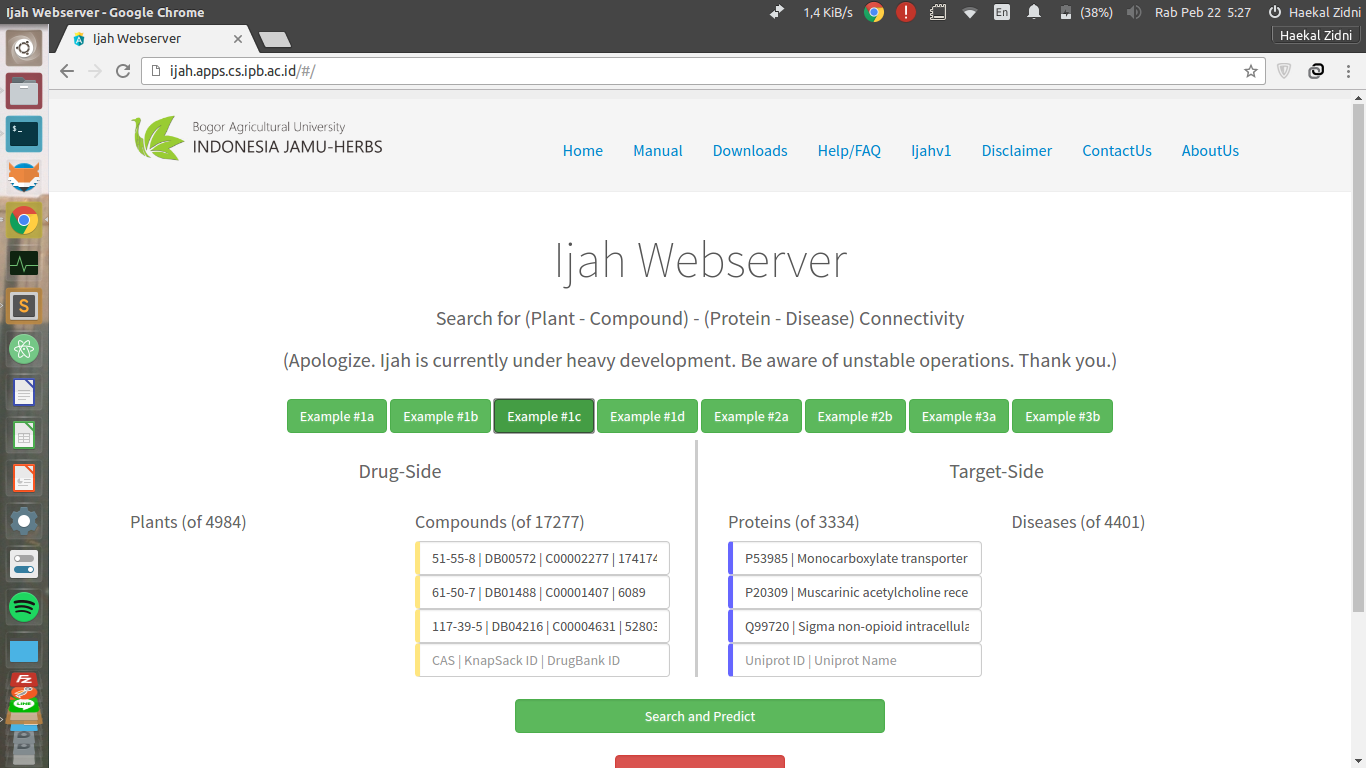
\includegraphics[scale=0.3]{example_1c.png}
% 	\caption{Example 1c}
% 	\label{fig:example_1c}
% \end{figure}

% Example 1c merupakan contoh use\-case pencarian antara Compounds di sisi Drug\-side dan Proteins pada Target\-side, merepresentasikan pencarian “Apakah senyawa yang diinputkan memiliki hubungan dengan protein yang diinputkan”. Hasil yang ditunjukkan adalah hubungan antara senyawa pada input dan protein pada input, termasuk tanaman dan penyakit yang terkait.

% \item \textbf{Example 1d}
% \begin{figure}[H]
% 	\centering
% 	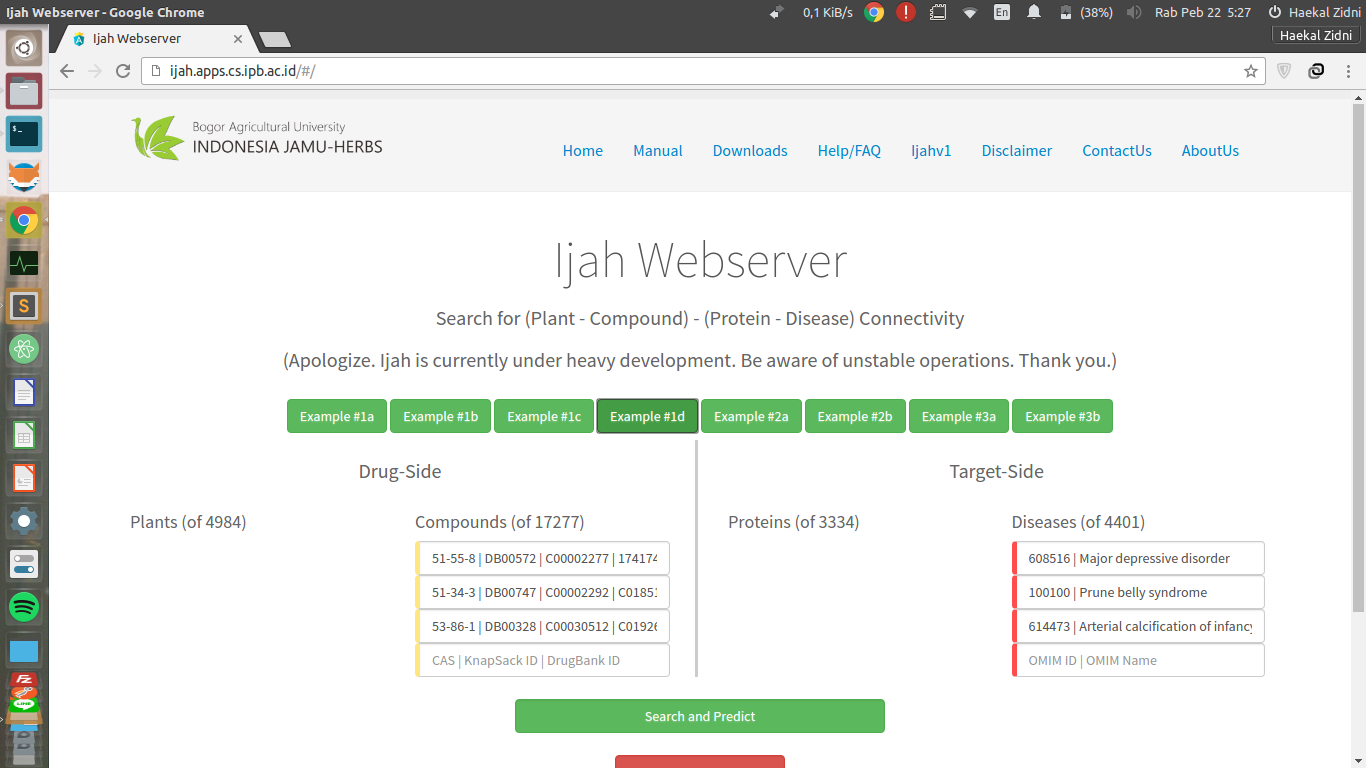
\includegraphics[scale=0.3]{example_1d.png}
% 	\caption{Example 1d}
% 	\label{fig:example_1d}
% \end{figure}

% Example 1d merupakan contoh use\-case pencarian antara Compounds di sisi Drug\-side dan Diseases pada Target\-side, merepresentasikan pencarian “Apakah senyawa yang diinputkan memiliki hubungan dengan penyakit yang diinputkan”. Hasil yang ditunjukkan yaitu berupa hubungan antara senyawa pada input dengan penyakit pada input, termasuk tanaman dan protein yang terkait.



% Example 2a merupakan contoh use\-case pencarian di sisi Drug\-side saja yaitu Plants. Hasil yang ditunjukkan adalah segala senyawa, protein, dan penyakit yang terkait pada tanaman yang diinputkan.

% \item \textbf{Example 2b}
% \begin{figure}[H]
% 	\centering
% 	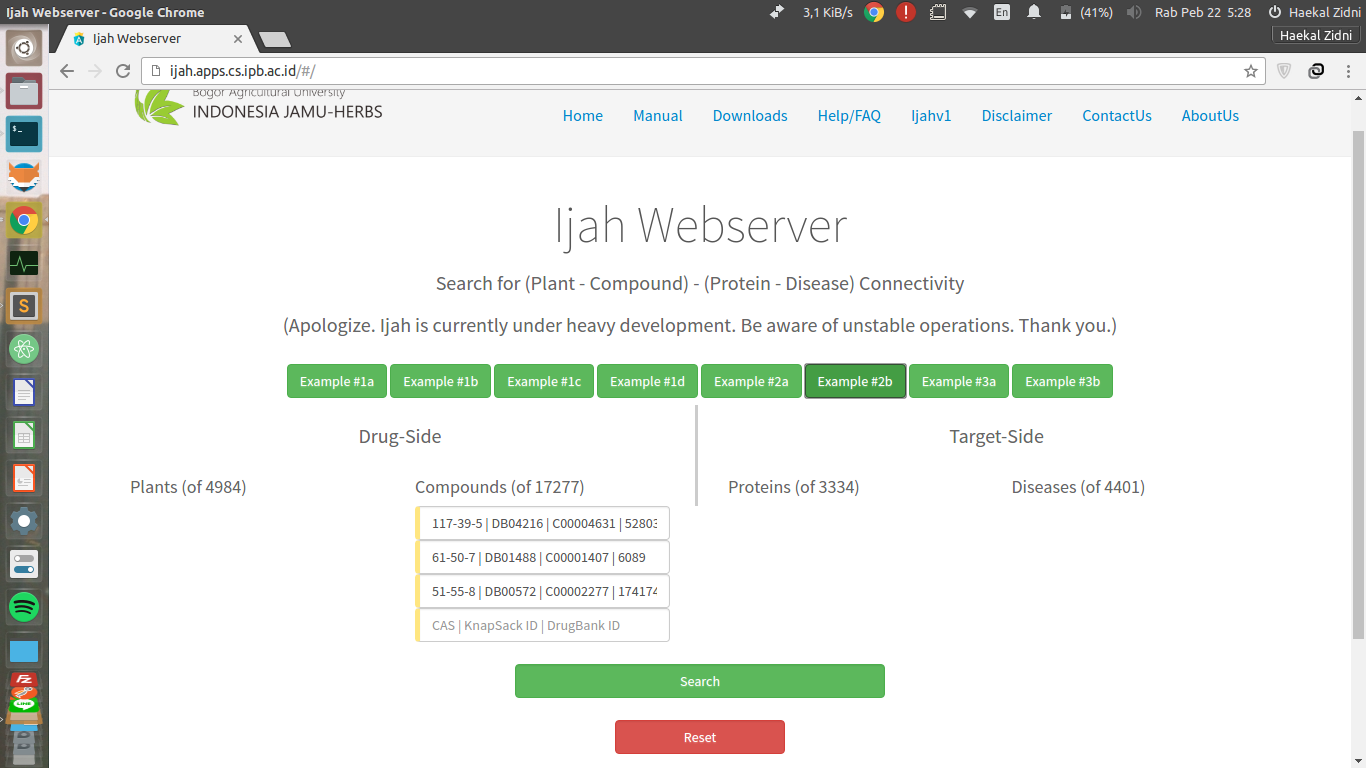
\includegraphics[scale=0.3]{example_2b.png}
% 	\caption{Example 2b}
% 	\label{fig:example_2b}
% \end{figure}

% Example 2b merupakan contoh use\-case pencarian di sisi Drug\-side saja yaitu Compounds. Hasil yang ditunjukkan adalah segala tanaman, protein, dan penyakit yang terkait pada senyawa yang diinputkan.

% \item \textbf{Example 3a}
% \begin{figure}[H]
% 	\centering
% 	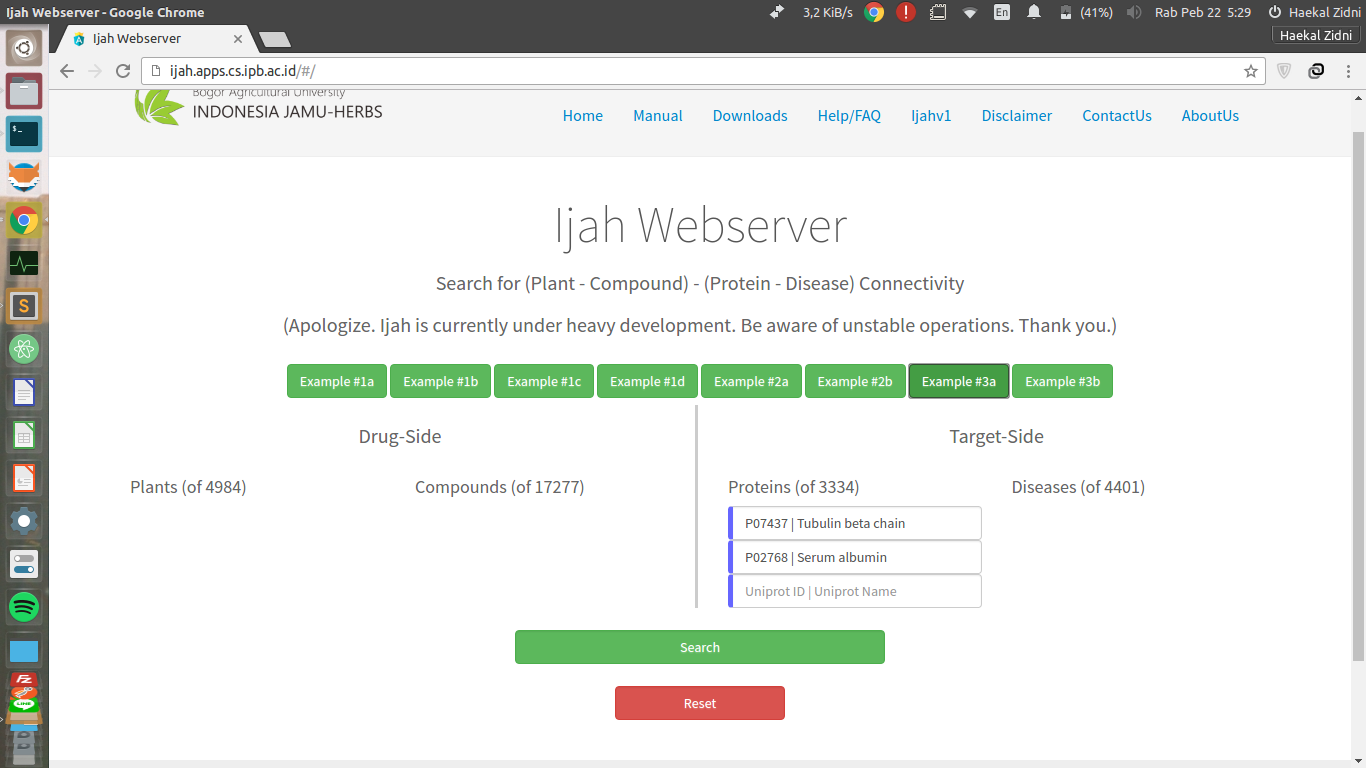
\includegraphics[scale=0.3]{example_3a.png}
% 	\caption{Example 3a}
% 	\label{fig:example_3a}
% \end{figure}

% Example 3a merupakan contoh use\-case pencarian di sisi Target\-side saja yaitu Proteins. Hasil yang ditunjukkan adalah segala tanaman, senyawa, dan penyakit yang terkait pada protein yang diinputkan.

% \item \textbf{Example 3b}
% \begin{figure}[H]
% 	\centering
% 	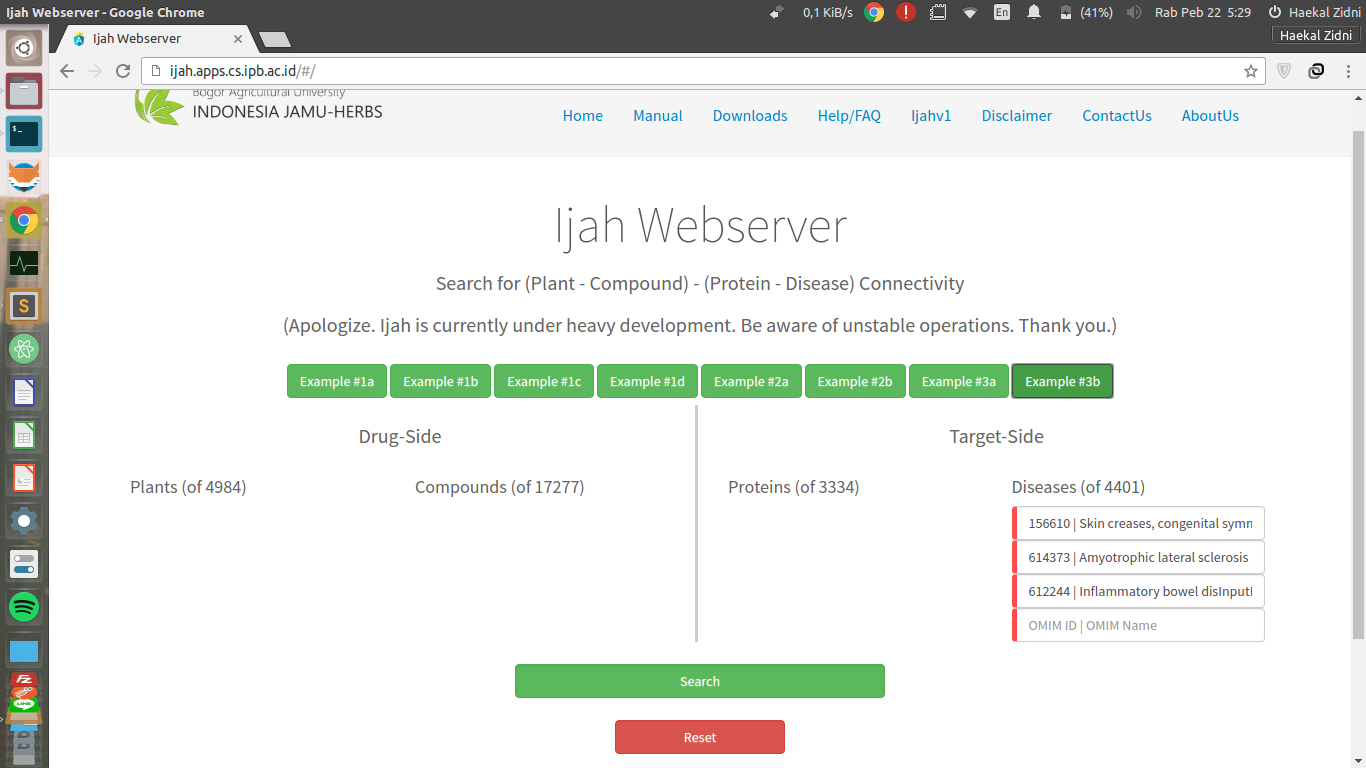
\includegraphics[scale=0.3]{example_3b.png}
% 	\caption{Example 3b}
% 	\label{fig:example_3b}
% \end{figure}

% Example 3b merupakan contoh use\-case pencarian di sisi Target\-side saja yaitu Diseases. Hasil yang ditunjukkan adalah segala tanaman, senyawa, dan protein yang terkait pada penyakit yang diinputkan.

% \end{enumerate}


% \subsection{Input Form}

% \begin{figure}[H]
% 	\centering
% 	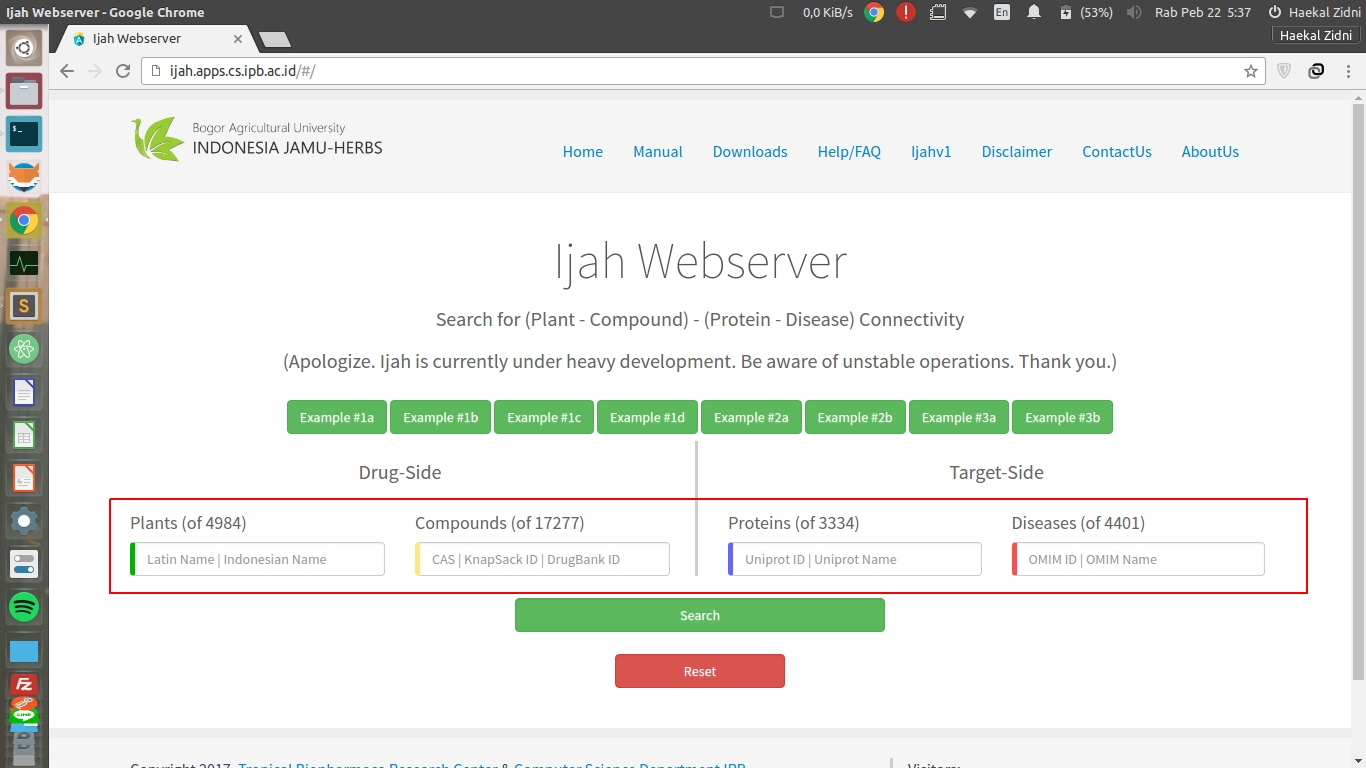
\includegraphics[scale=0.3]{ijah_input_row.png}
% 	\caption{Barisan kotak input Ijah Webserver}
% 	\label{fig:ijah_input_row}
% \end{figure}

% Setiap Example diatas merupakan kumpulan \emph{predefined input}. Selain input melalui Examples, tentunya input manual tetap dapat dilakukan. Setiap input memiliki fitur \emph{auto\-completion} untuk menghindari kesalahan.

% \begin{figure}[H]
% 	\centering
% 	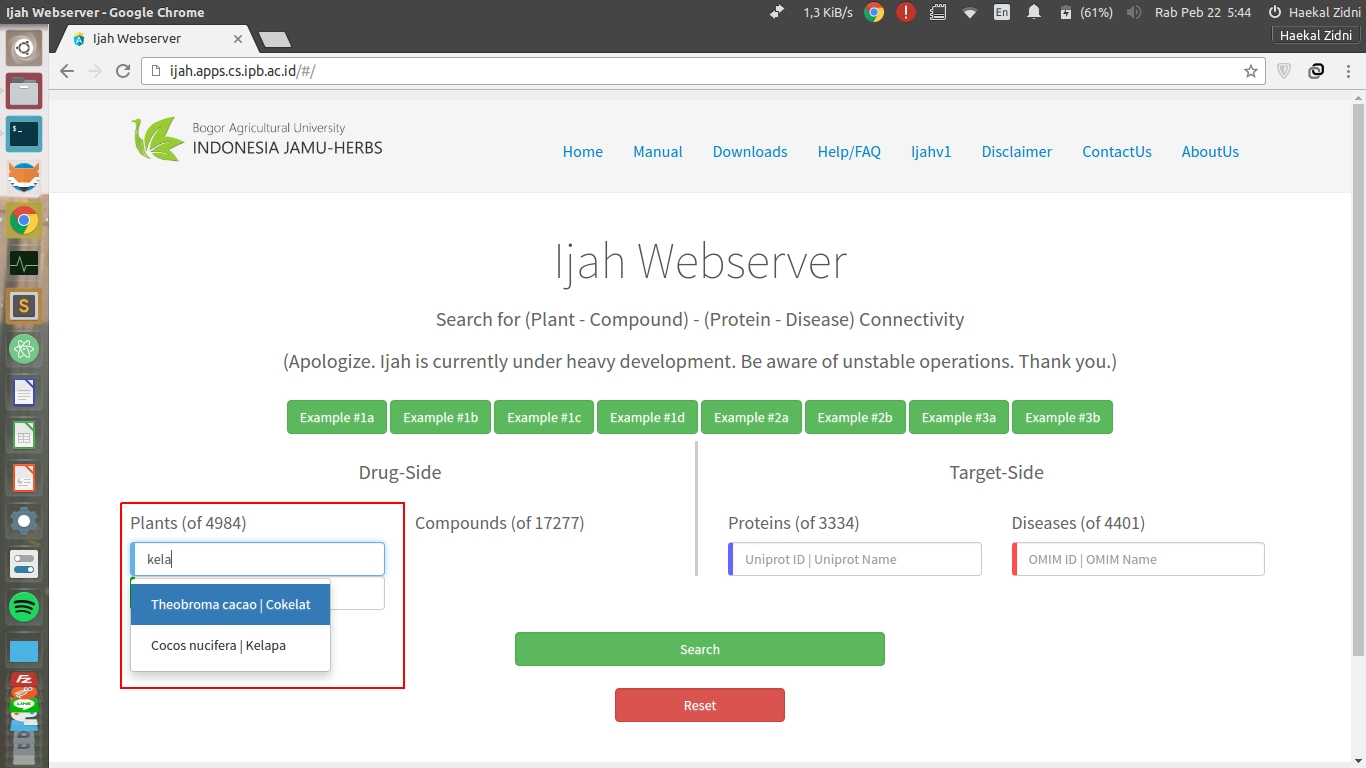
\includegraphics[scale=0.3]{ijah_autocomplete.png}
% 	\caption{\emph{Auto\-completion} pada Ijah Webserver}
% 	\label{fig:ijah_autocomplete}
% \end{figure}

% \textbf{Penting:} untuk memasukkan input tidak bisa hanya diketik, namun jika \emph{autocomplete} telah menunjukkan input yang sesuai, maka suggestion pada \emph{autocomplete} harus di\-klik. Sebagai contoh jika kita ingin melakukan pencarian untuk kelapa, maka klik “Cocos nucifera | Kelapa”.

% \begin{figure}[H]
% 	\centering
% 	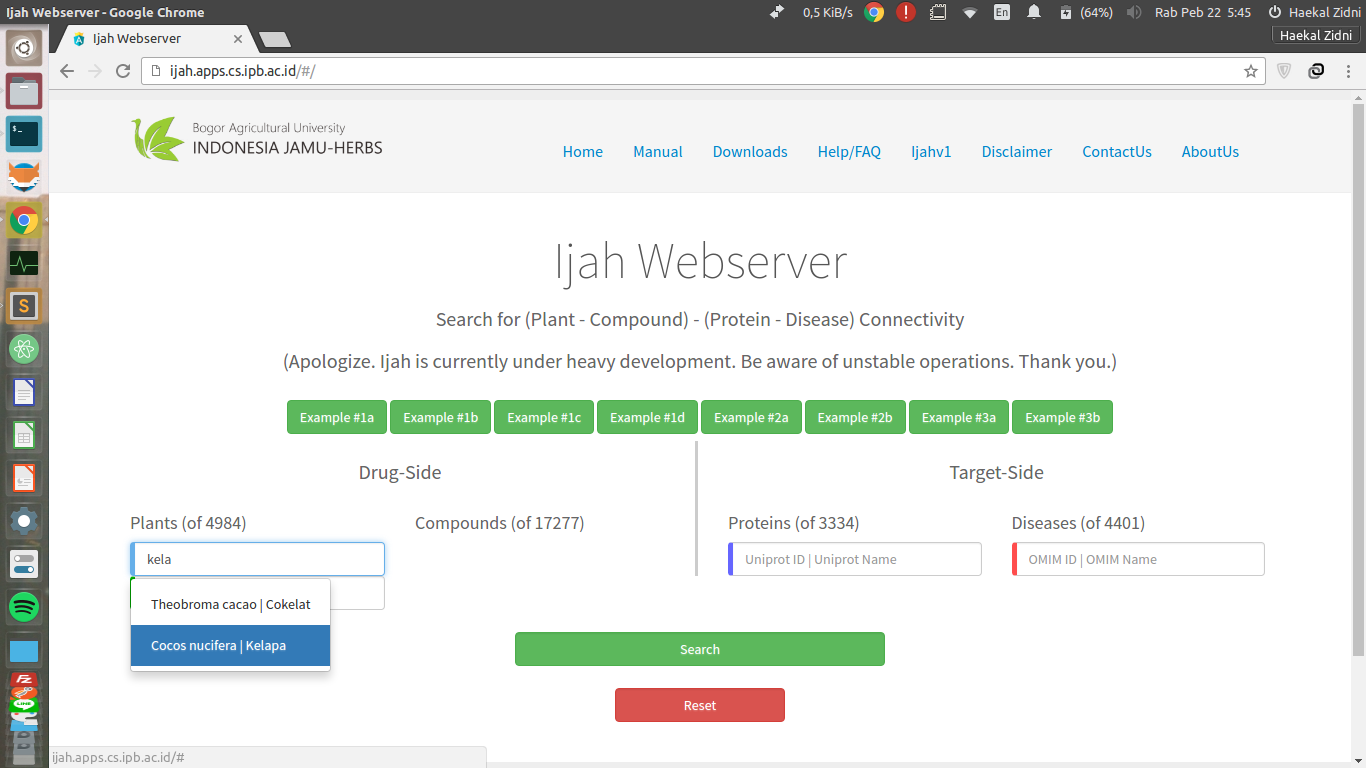
\includegraphics[scale=0.3]{ijah_autocomplete_click.png}
% 	\caption{Sorot dan klik hasil yang dimaksud untuk memasukkannya pada input}
% 	\label{fig:ijah_autocomplete_click}
% \end{figure}

% Setelah di\-klik maka input akan terlengkapi

% \begin{figure}[H]
% 	\centering
% 	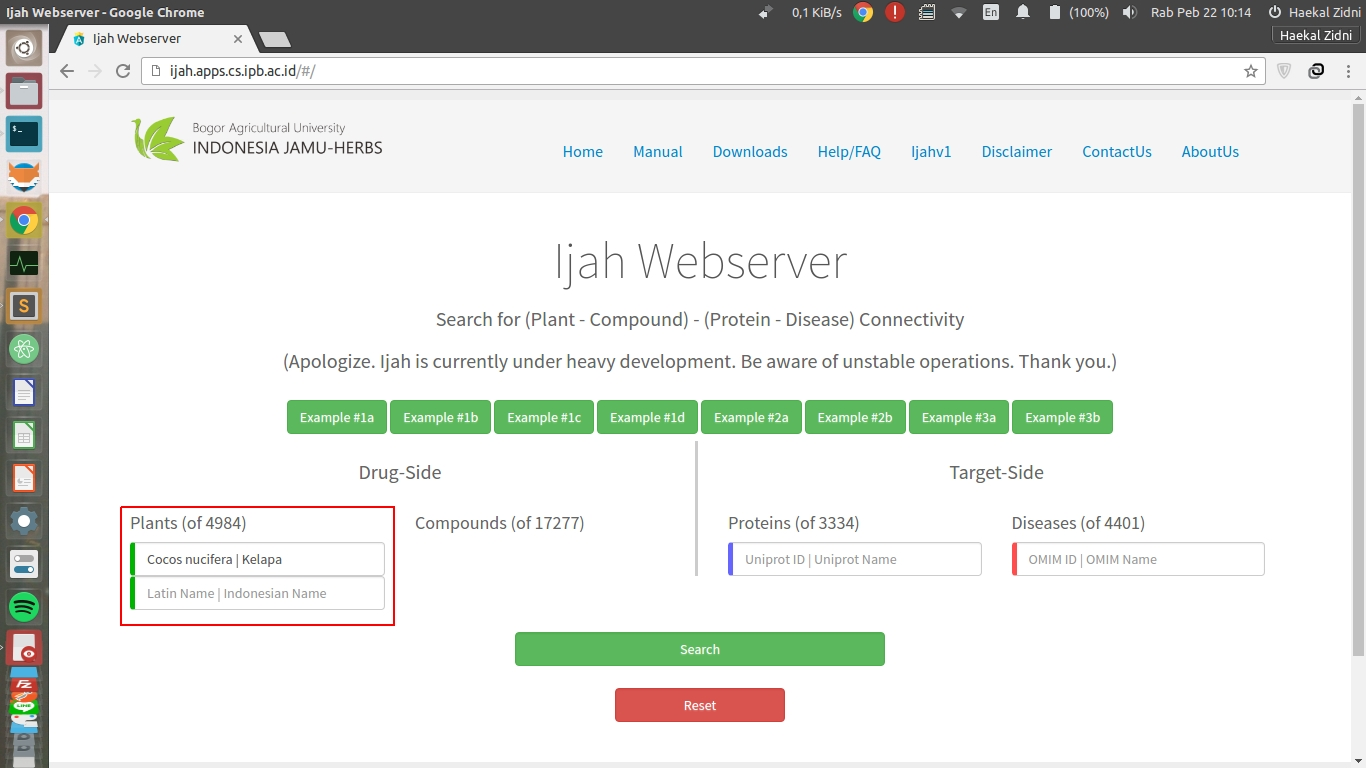
\includegraphics[scale=0.3]{ijah_autocomplete_complete.png}
% 	\caption{Setelah diklik input akan terlengkapi}
% 	\label{fig:ijah_autocomplete_complete}
% \end{figure}

% \textbf{Penting:} Pada tiap sisi (Drug\-side atau Target\-side) hanya bisa memilih salah satu dari dua input pada tiap side. Misal ketika memilih Plants ada Drug\-side, maka Compounds akan secara otomatis ter\-disable, begitu pula sebaliknya. Hal yang sama berlaku pada Target\-side. Hal ini dimaksudkan untuk menjaga konsistensi output, mencegah adanya input yang invalid misalkan tanaman dan senyawa yang sama sekali tidak berhubungan (senyawa yang diinputkan tidak ada pada tanaman yang diinputkan).

% Setelah input selesai (misalkan pada contoh ini kita hanya melakukan  \emph{search} untuk semua senyawa, protein, dan penyakit yang terkait pada tanaman kelapa dan sambiloto), klik \textbf{Search}

% \begin{figure}[H]
% 	\centering
% 	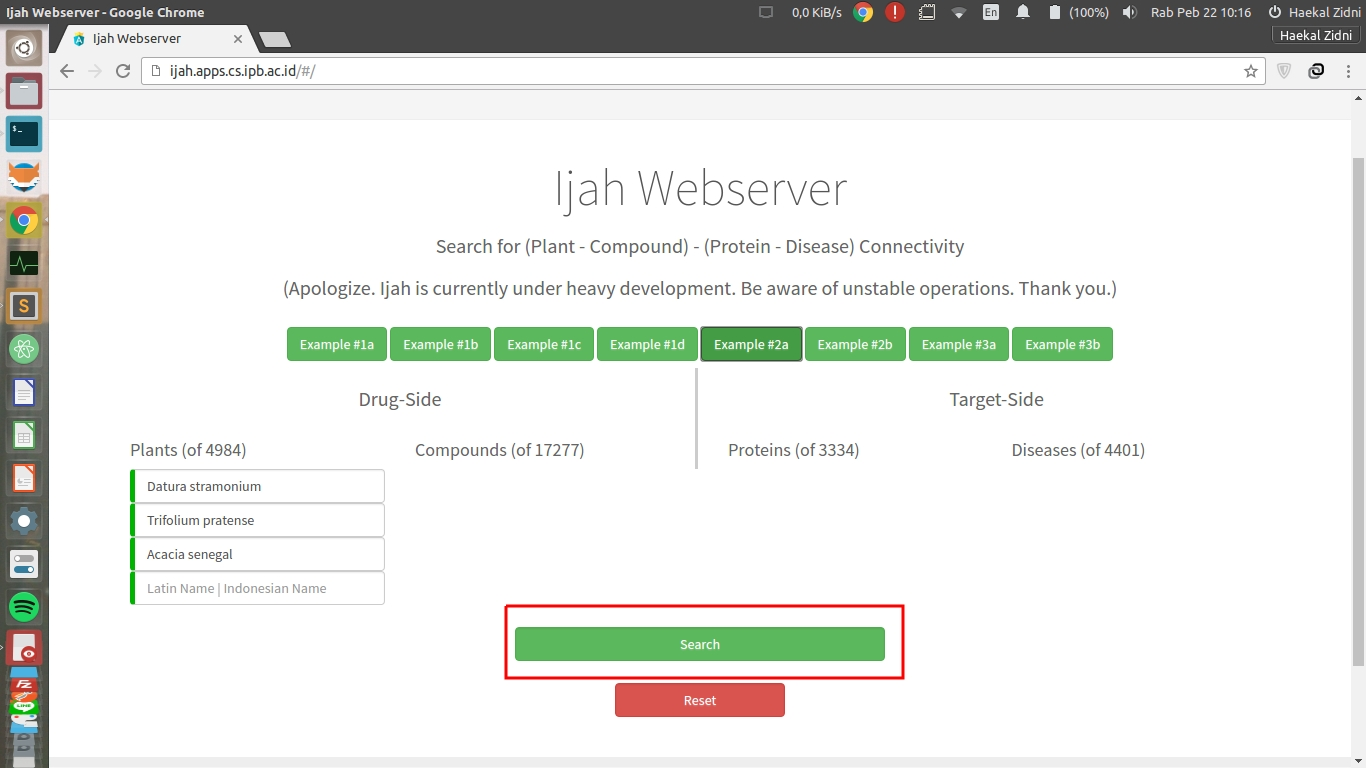
\includegraphics[scale=0.3]{ijah_searchonly.png}
% 	\caption{Mode \emph{search only}}
% 	\label{fig:ijah_searchonly}
% \end{figure}

% \textbf{Catatan:} Jika input berada hanya dari satu sisi (Drug\-side saja atau Target\-side saja) maka tombol akan bertuliskan \textbf{Search}. Jika input berasal dari kedua sisi maka tombol akan berubah menjadi \textbf{Search and Predict}, seperti contoh berikut

% \begin{figure}[H]
% 	\centering
% 	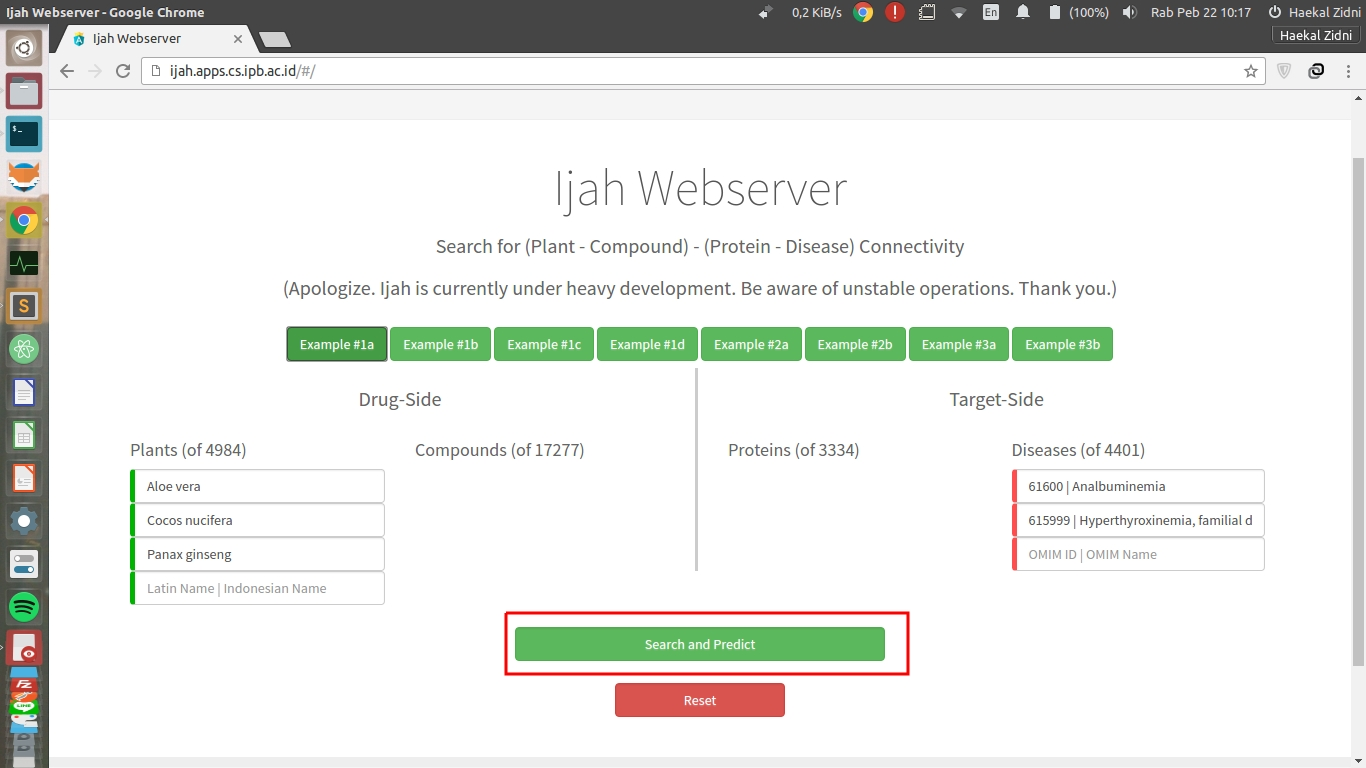
\includegraphics[scale=0.3]{ijah_search_predict.png}
% 	\caption{Mode  \emph{search and predict}}
% 	\label{fig:ijah_search_predict}
% \end{figure}

% Untuk mengosongkan semua input dapat mengklik tombol Reset

% \begin{figure}[H]
% 	\centering
% 	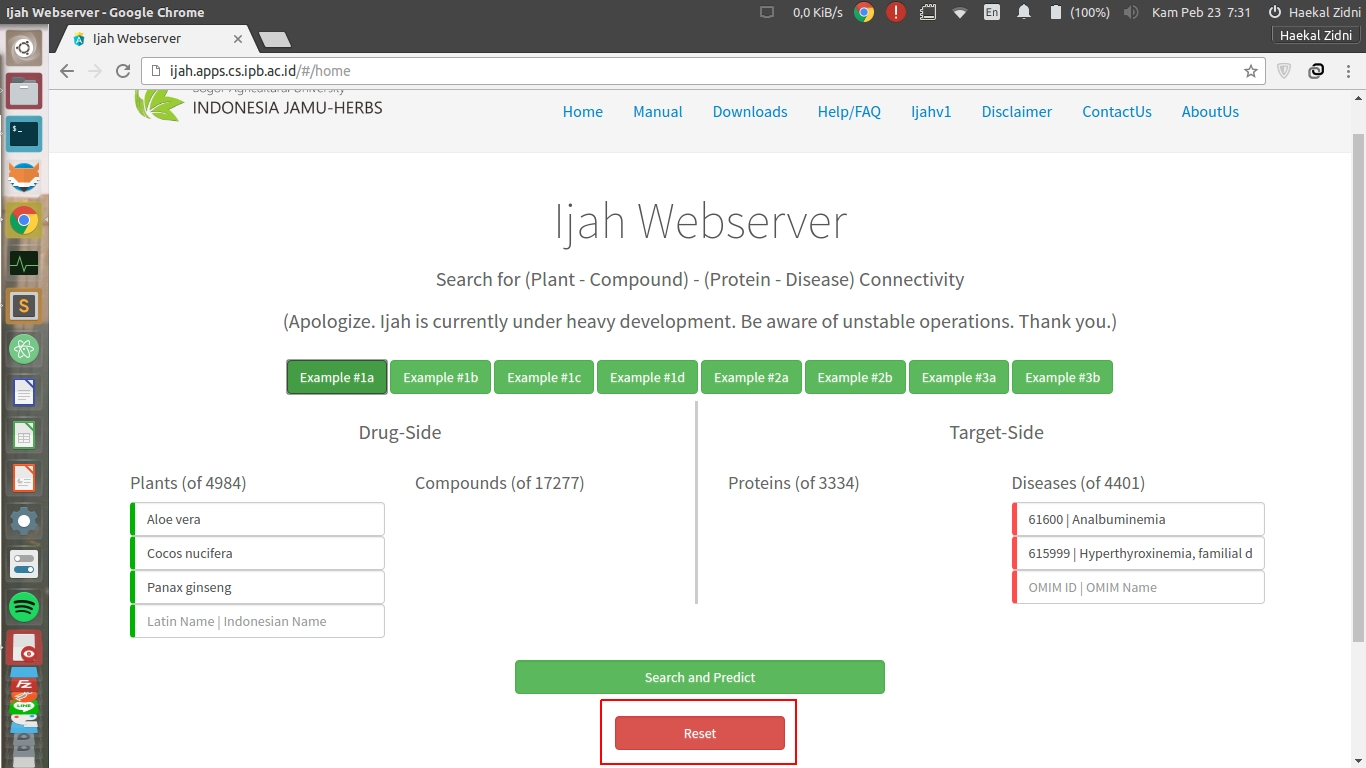
\includegraphics[scale=0.3]{ijah_inputreset.png}
% 	\caption{Tombol \emph{reset} untuk mengosongkan input kembali}
% 	\label{fig:ijah_inputreset}
% \end{figure}

% \section{Output} 

% \textbf{Asumsi:} menggunakan input \emph{search\-only} pada tanaman Kelapa (Cocos Nucifera) dan Sambiloto (Andrographis Paniculata)

% \begin{figure}[H]
% 	\centering
% 	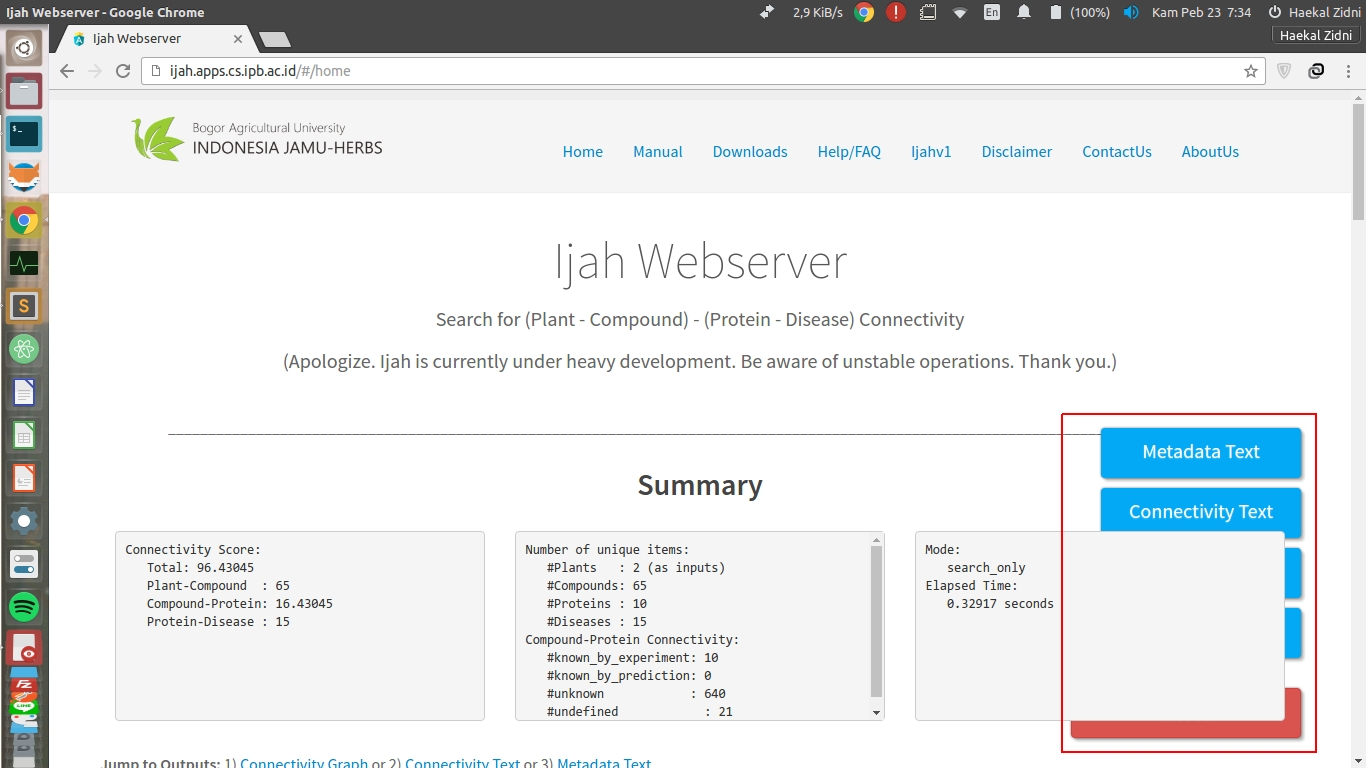
\includegraphics[scale=0.3]{ijah_floatingbutton.png}
% 	\caption{\emph{Floating button} yang tertutupi}
% 	\label{fig:ijah_floatingbutton}
% \end{figure}

% \textbf{Catatan:} pada resolusi yang lebih rendah dari 1920x1080 piksel (umumnya 1366x768 piksel) maka tombol biru untuk jump ke setiap jenis output akan tertutup oleh output itu sendiri.

% Jika dirasa kurang nyaman, maka hal ini dapat diatasi dengan meng\-klik ikon Options berupa tiga titik di pojok kanan atas pada Google Chrome

% \begin{figure}[H]
% 	\centering
% 	
\includegraphics[scale=0.3]{chrome_options.png}
% 	\caption{Tombol \emph{Settings/More Options} pada Chrome}
% 	\label{fig:chrome_options}
% \end{figure}

% Lalu setelah opsi terbuka, cari menu Zoom



% \subsection{Output Summary}

% \begin{figure}[H]
% 	\centering
% 	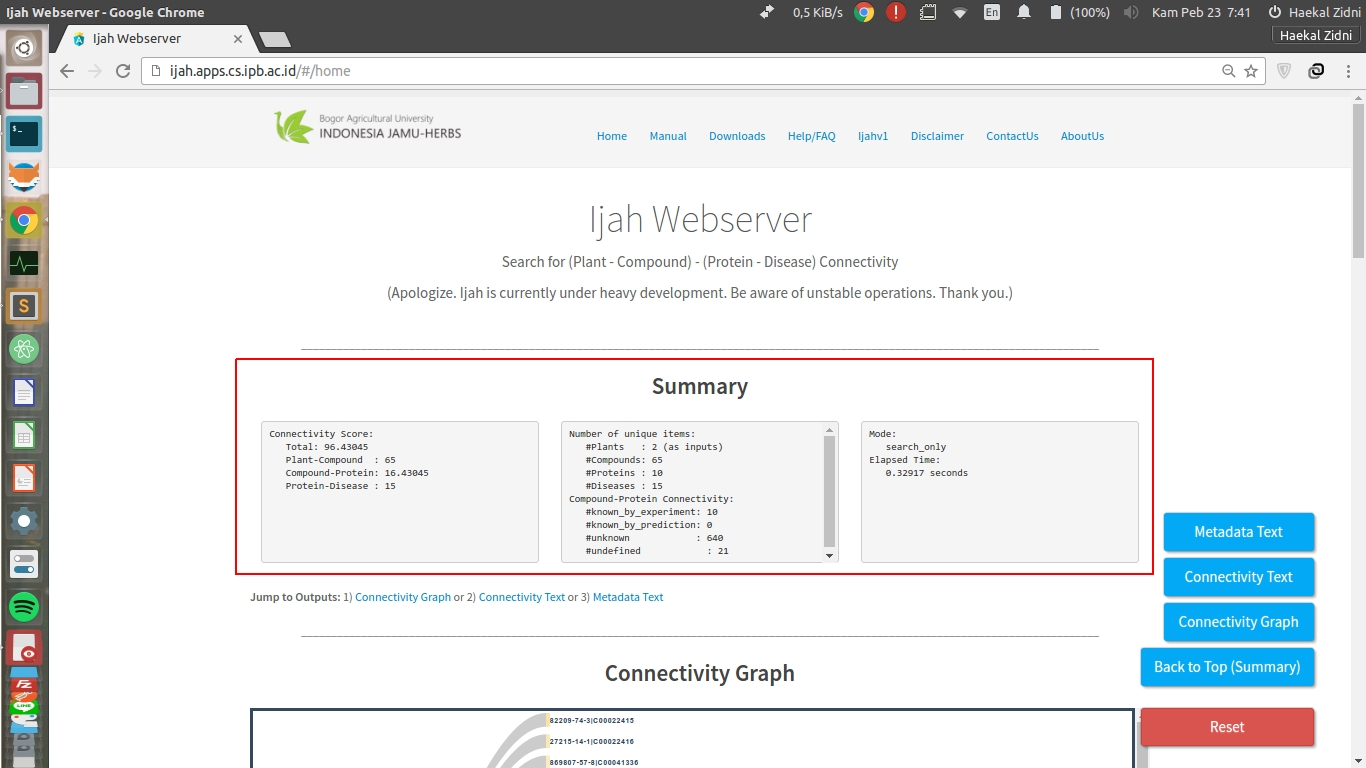
\includegraphics[scale=0.3]{ijah_output_summary.png}
% 	\caption{Output Summary pada Ijah Webserver}
% 	\label{fig:ijah_output_summary}
% \end{figure}

% \textbf{Summary} berisikan ringkasan hasil output:
% \begin{itemize}
% 	\item Connectivity Score menunjukkan skor keterhubungan antara setiap komponen, dimana bernilai 1 jika terhubung dan 0 jika tidak terhubung, dan berupa nilai antara 0 dan 1 jika nilai keterhubungan tidak eksak (misal hasil dari  \emph{predictor}). Pada contoh ini setiap keterhubungan bernilai 1 sehingga jumlahnya akan sama dengan jumlah total keterhubungan komponen.
% 	\item Number of unique items menunjukkan jumlah \emph{item} yang unik yang ditunjukkan pada output.
% 	\item Compound\-Protein connectivity menunjukkan jumlah hubungan antara senyawa dan protein pada output. Terbagi menjadi hasil \emph{known by experiment} (data merupakan hasil eksperimen terpercaya dan sudah ada dalam database) dan \emph{known by prediction} (data merupakan hasil prediksi dari  \emph{predictor}).
% 	\item Mode yaitu mode pencarian, apakah hanya pencarian (search only) atau pencarian dan prediksi (search and predict).
% 	\item Elapsed Time menunjukkan waktu yang digunakan untuk mengolah output (melakukan pencarian atau prediksi).
% \end{itemize}

% Output terdiri dari \textbf{Connectivity graph} (graf \emph{bipartite} keterhubungan), \textbf{Connectivity text} (berupa teks untuk keterhubungan), dan \textbf{Metadata Text} (berupa teks berisi \emph{item} yang terlibat).

% Untuk langsung menuju salah satu jenis output dapat melalui klik pada \textbf{Jump} To atau tombol\-tombol biru di sisi kanan bawah.



% Sedangkan tombol \textbf{Reset} berguna untuk mengosongkan semua output dan kembali pada Input

% \begin{figure}[H]
% 	\centering
% 	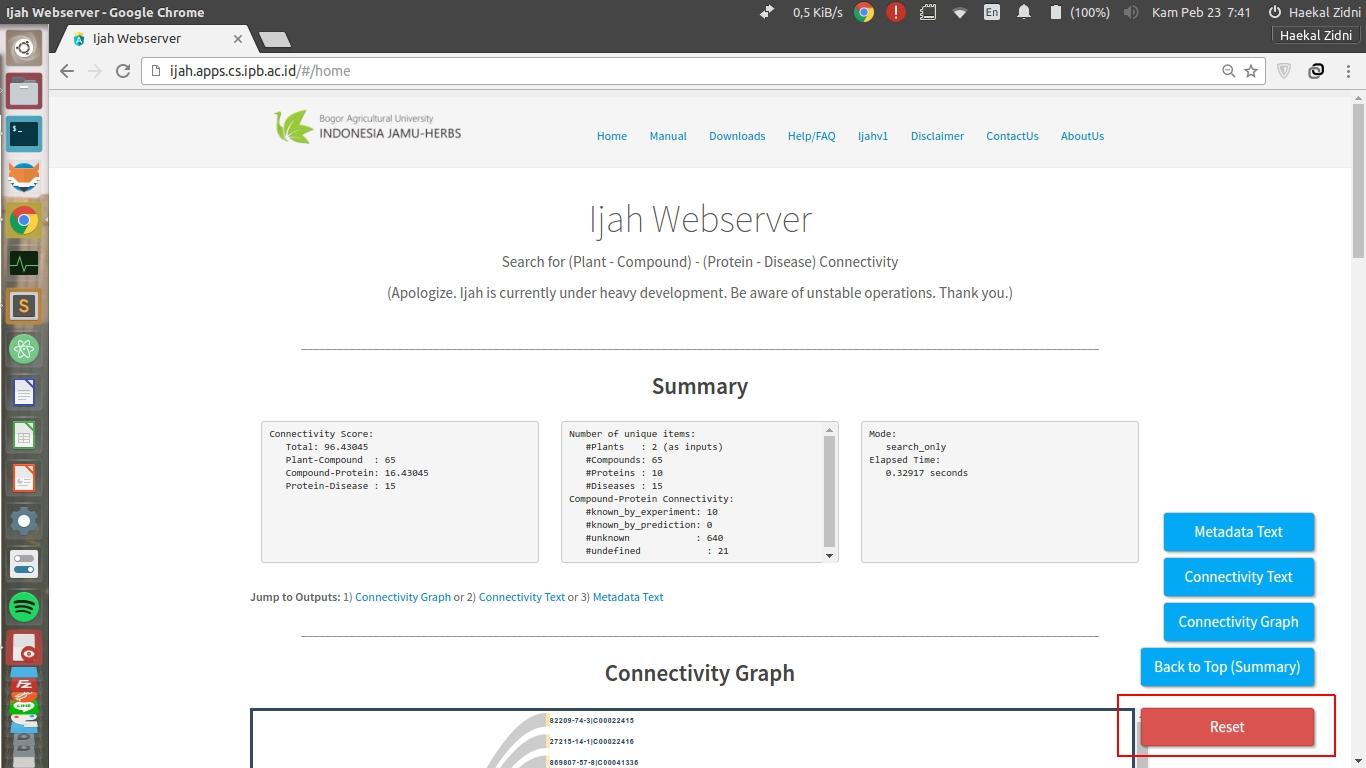
\includegraphics[scale=0.3]{ijah_outputreset.png}
% 	\caption{Tombol \emph{Reset} untuk mengosongkan dan kembali ke posisi awal Home}
% 	\label{fig:ijah_outputreset}
% \end{figure}

% \subsection{Connectivity Graph}

% \begin{figure}[H]
% 	\centering
% 	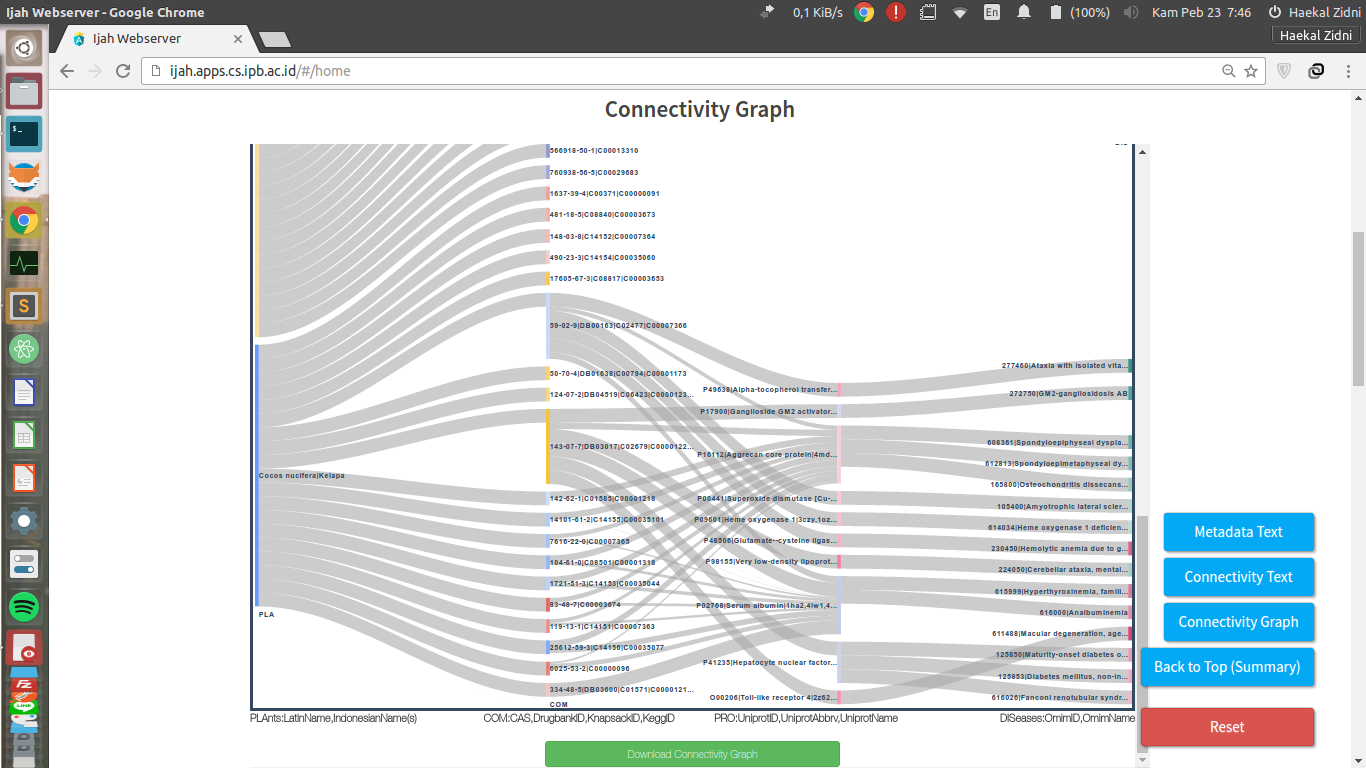
\includegraphics[scale=0.3]{ijah_graph.png}
% 	\caption{Tampilan \emph{Multipartite Connectivity Graph}}
% 	\label{fig:ijah_graph}
% \end{figure}

% Output Connectivity Graph merupakan keluaran berupa graf yang menyatakan keterhubungan setiap komponen, antara tanaman dengan senyawa, senyawa dengan protein, dan protein dengan penyakit. Graf ini dapat di\-scroll secara vertikal (atas dan bawah). Pada contoh diatas, jika ada graf yang terputus (misal pada senyawa tertentu tidak ada lanjutannya) berarti data keterkaitan protein pada senyawa tersebut tidak tersedia.

% \begin{figure}[H]
% 	\centering
% 	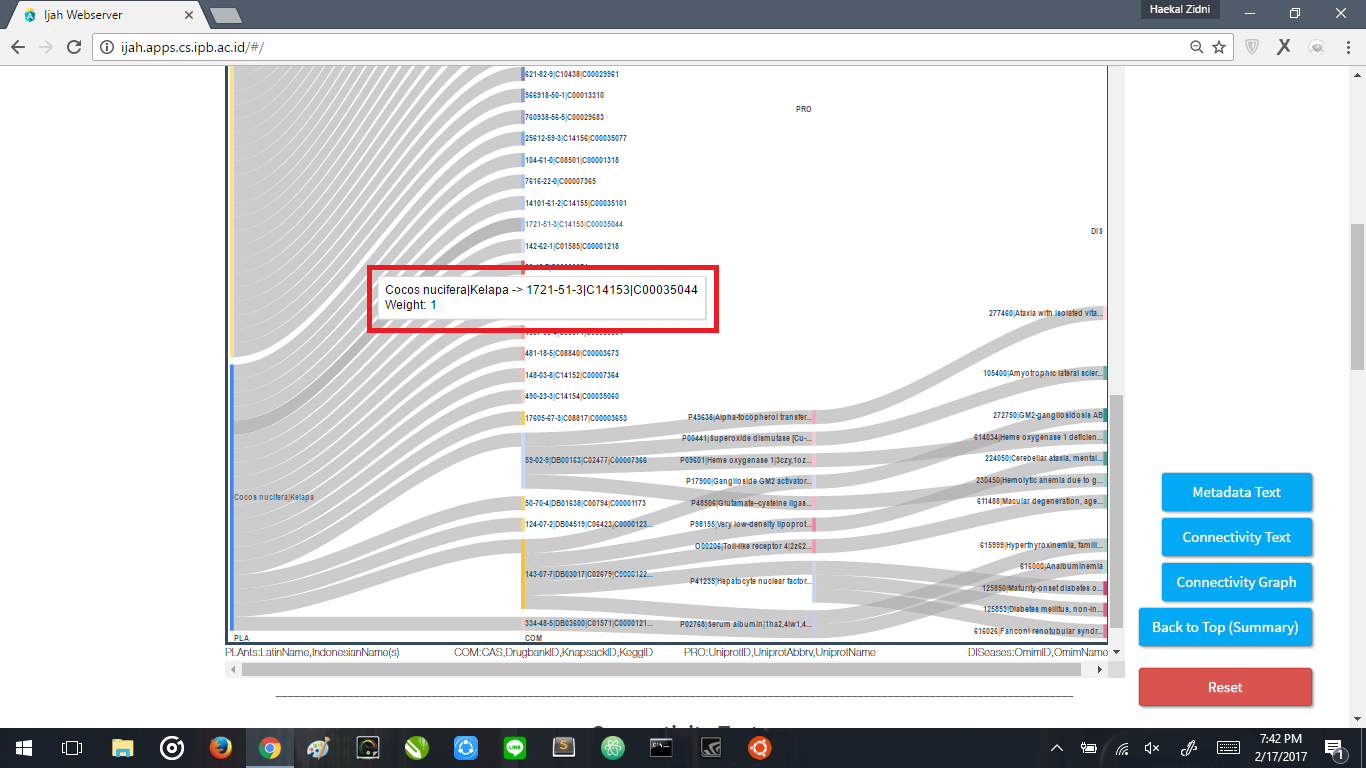
\includegraphics[scale=0.3]{ijah_graph_tooltip.png}
% 	\caption{Pop\-up Info Konektivitas}
% 	\label{fig:ijah_graph_tooltip}
% \end{figure}

% Jika salah satu garis graf disorot, maka akan muncul info keterkaitan dari garis graf yang disorot, serta skor keterhubungannya. 

% Gambar utuh \emph{Connectivity Graph} dapat di\-download melalui tombol \textbf{Download Connectivity Graph} di bawah graf

% \begin{figure}[H]
% 	\centering
% 	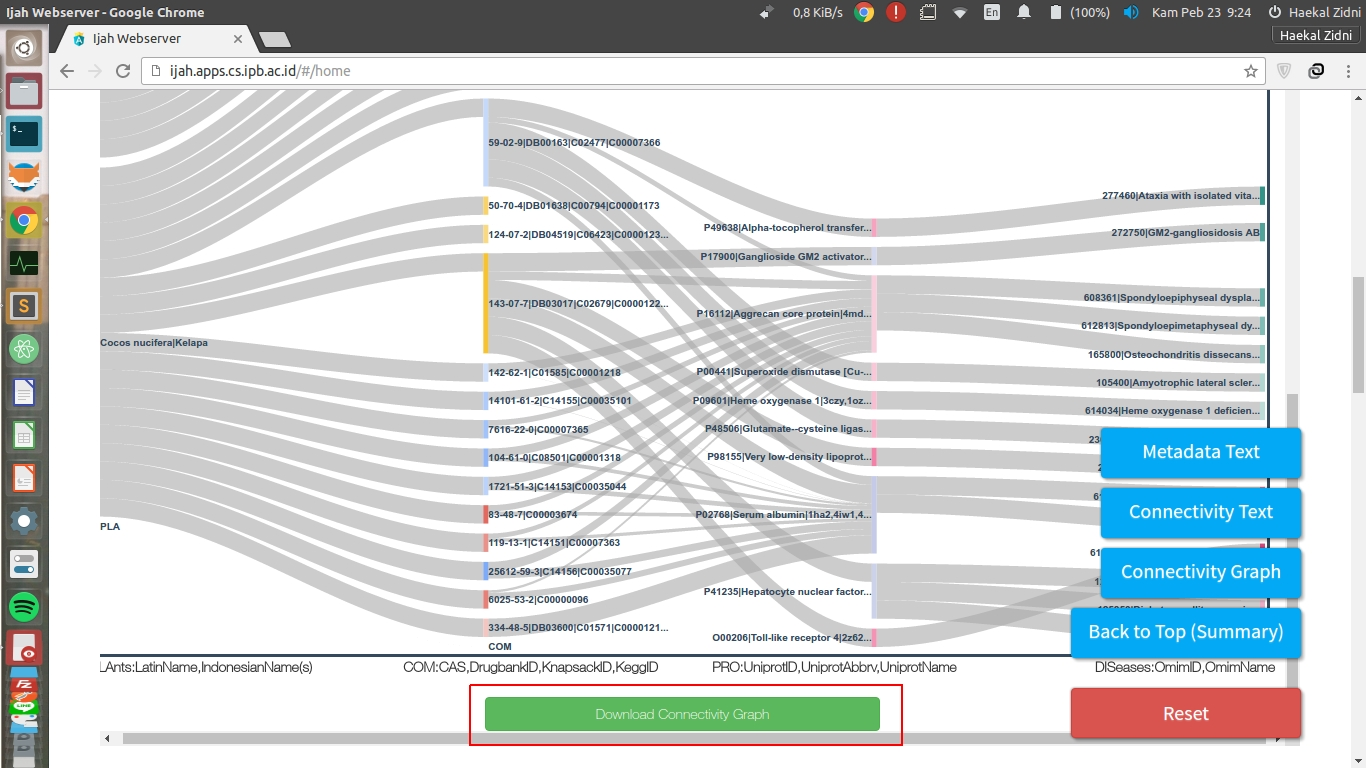
\includegraphics[scale=0.3]{ijah_graph_download.png}
% 	\caption{Tombol Download untuk mengunduh file \emph{Connectivity Graph Output}}
% 	\label{fig:ijah_graph_download}
% \end{figure}

% \textbf{Memahami Data Output}
% Pada Plants (tanaman) data berupa nama latin dan nama Indonesia dari tanaman tersebut. Pada Compounds (senyawa) data berupa ID CAS, ID DrugBank, ID KnapSack, dan ID Kegg dari senyawa tersebut. Pada Proteins, data berupa ID Uniprot, singkatan Uniprot (abbreviation), dan nama Uniprot dari protein tersebut. Pada Diseases (penyakit), data berupa ID Omim dan nama Omim dari penyakit tersebut. Weight merupakan skor keterhubungan antara dua komponen tersebut.

% \subsection{Connectivity Text}

% \begin{figure}[H]
% 	\centering
% 	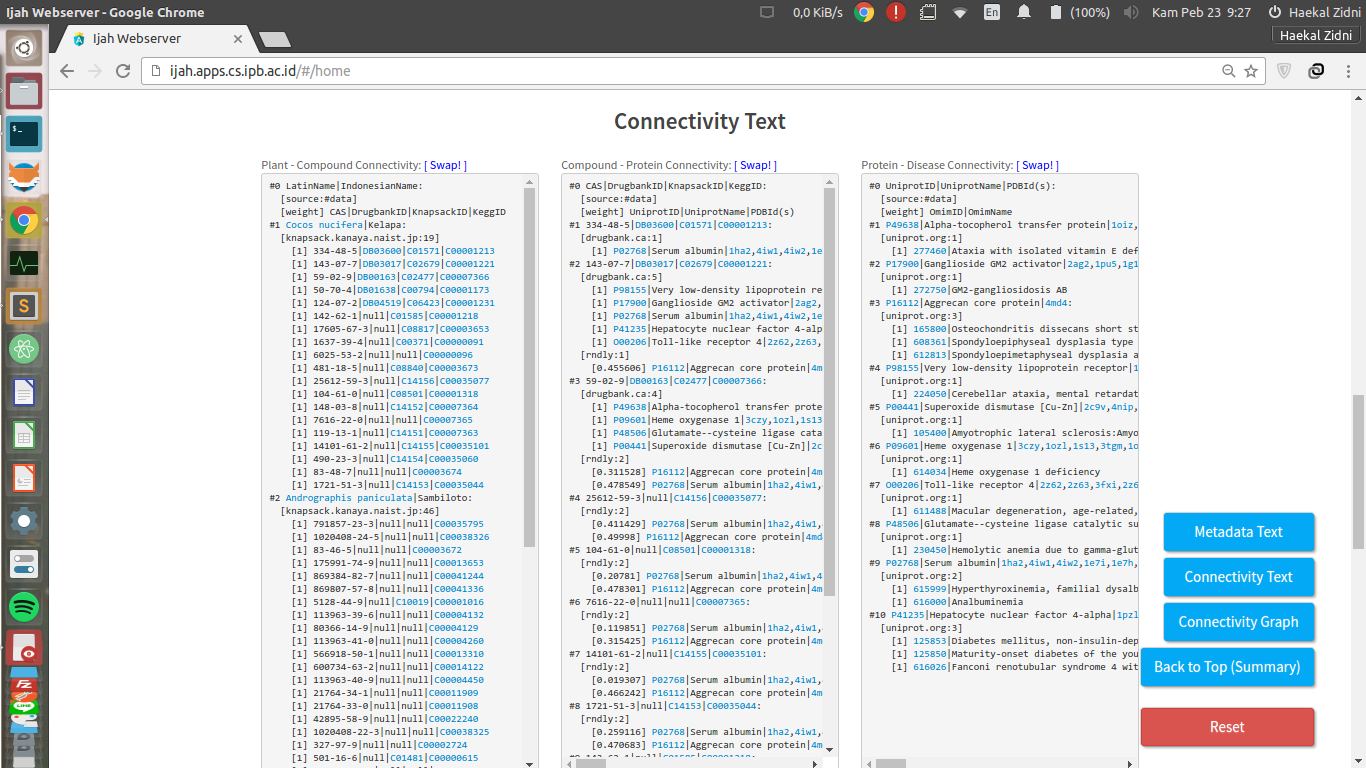
\includegraphics[scale=0.3]{ijah_text.png}
% 	\caption{Tampilan \emph{Connectivity Text Output}}
% 	\label{fig:ijah_text}
% \end{figure}

% Output Connectivity Text berupa output yang sama yang disajikan dalam bentuk teks. Untuk penerjemahan data dapat dilihat di atas pada bagian Memahami Data Output.

% \begin{figure}[H]
% 	\centering
% 	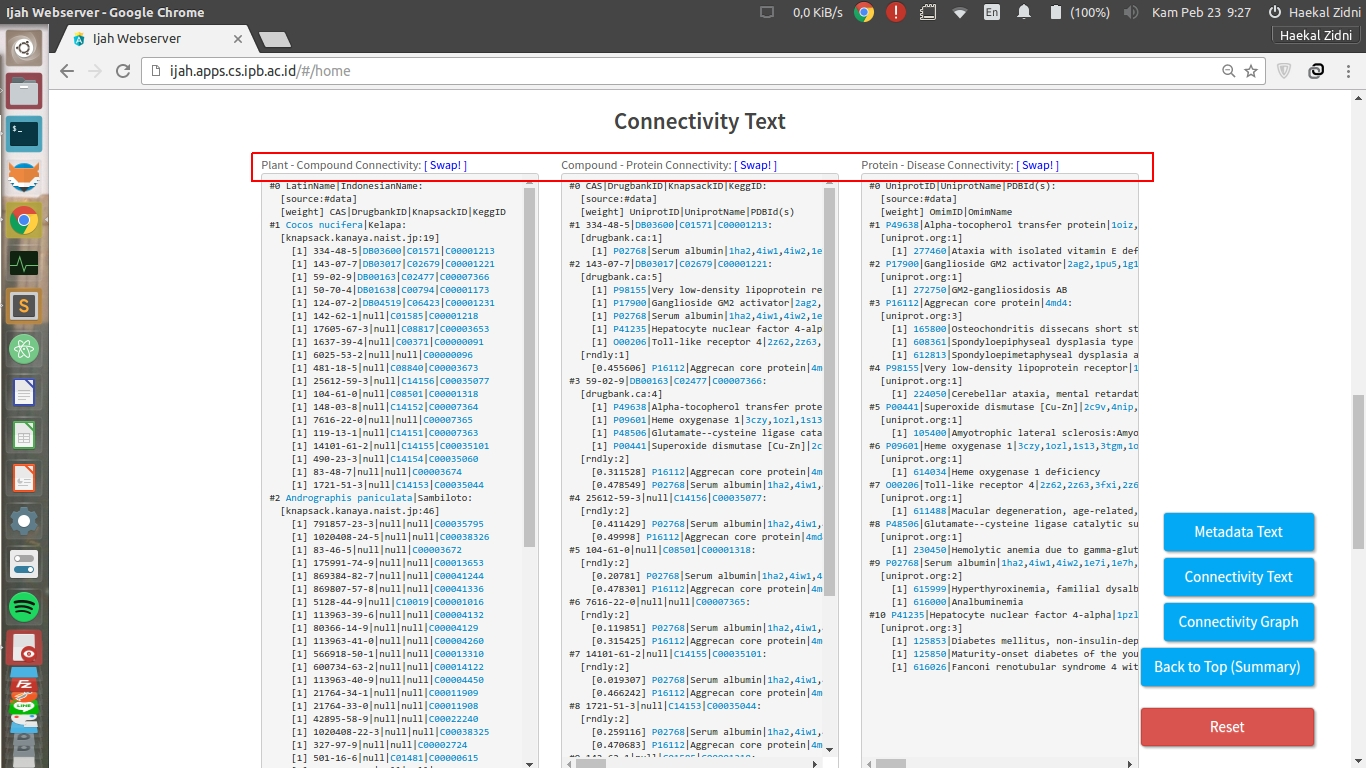
\includegraphics[scale=0.3]{ijah_text_swap.png}
% 	\caption{Tombol \emph{Swap} untuk membalik posisi item pada output}
% 	\label{fig:ijah_text_swap}
% \end{figure}

% Pada Connectivity Text, output yang menunjukkan hubungan antara Plant\-Compound, Compound\-Protein dan Protein\-Disease dapat dibalik. Misal Plant\-Compound dibalik menjadi Compound\-Plant, dengan cara mengklik Swap pada bagian atas text output. Hasil swap ditunjukkan pada contoh gambar dibawah:

% \begin{figure}[H]
% 	\centering
% 	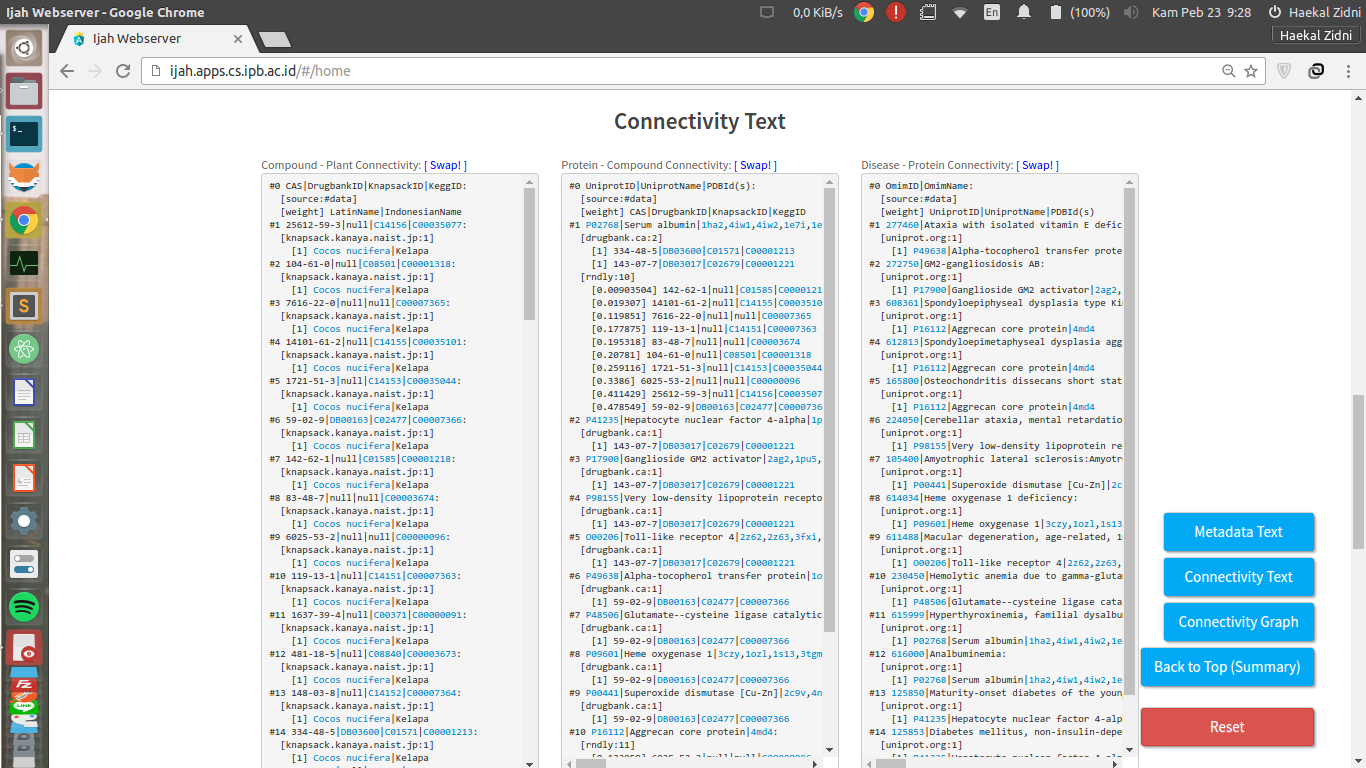
\includegraphics[scale=0.3]{ijah_text_swapresult.png}
% 	\caption{Hasil \emph{swapping} item pada output}
% 	\label{fig:ijah_text_swapresult}
% \end{figure}

% Pada text output ini, dapat dilakukan scroll baik secara vertikal (atas\-bawah) maupun horizontal (kiri\-kanan). Isi \emph{Connectivity Text Output} ini juga dapat di\-download



% \subsection{Metadata Text}

% \begin{figure}[H]
% 	\centering
% 	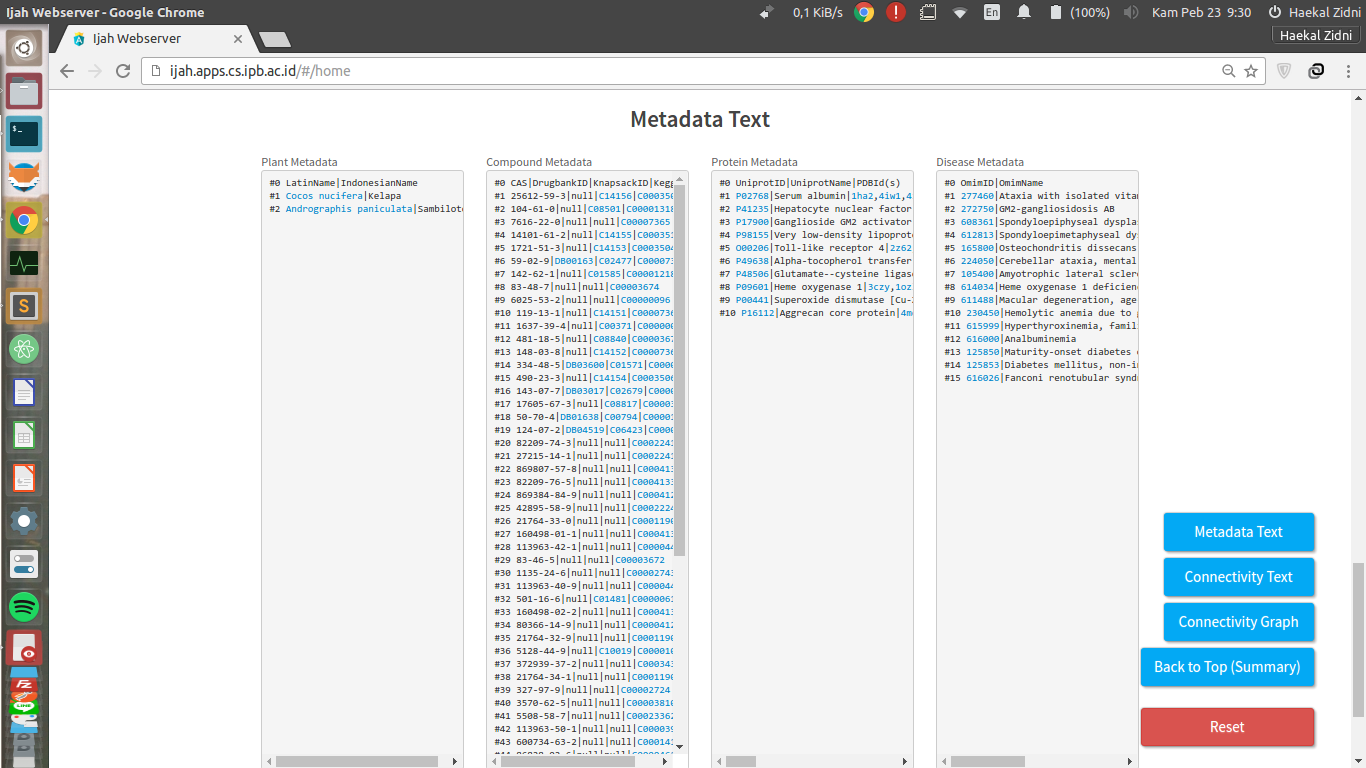
\includegraphics[scale=0.3]{ijah_meta.png}
% 	\caption{Tampilan \emph{Metadata Text Output}}
% 	\label{fig:ijah_meta}
% \end{figure}

% Output Metadata Text berisikan metadata dari item\-item yang terlibat (baik item yang dijadikan input, maupun item yang memiliki keterhubungan dengan input tersebut sebagai hasil pencarian keterhubungan). Metadata yang tersedia dapat di\-download sebagai file teks dengan mengklik tombol download yang tersedia dibawah output Metadata Text:

% \begin{figure}[H]
% 	\centering
% 	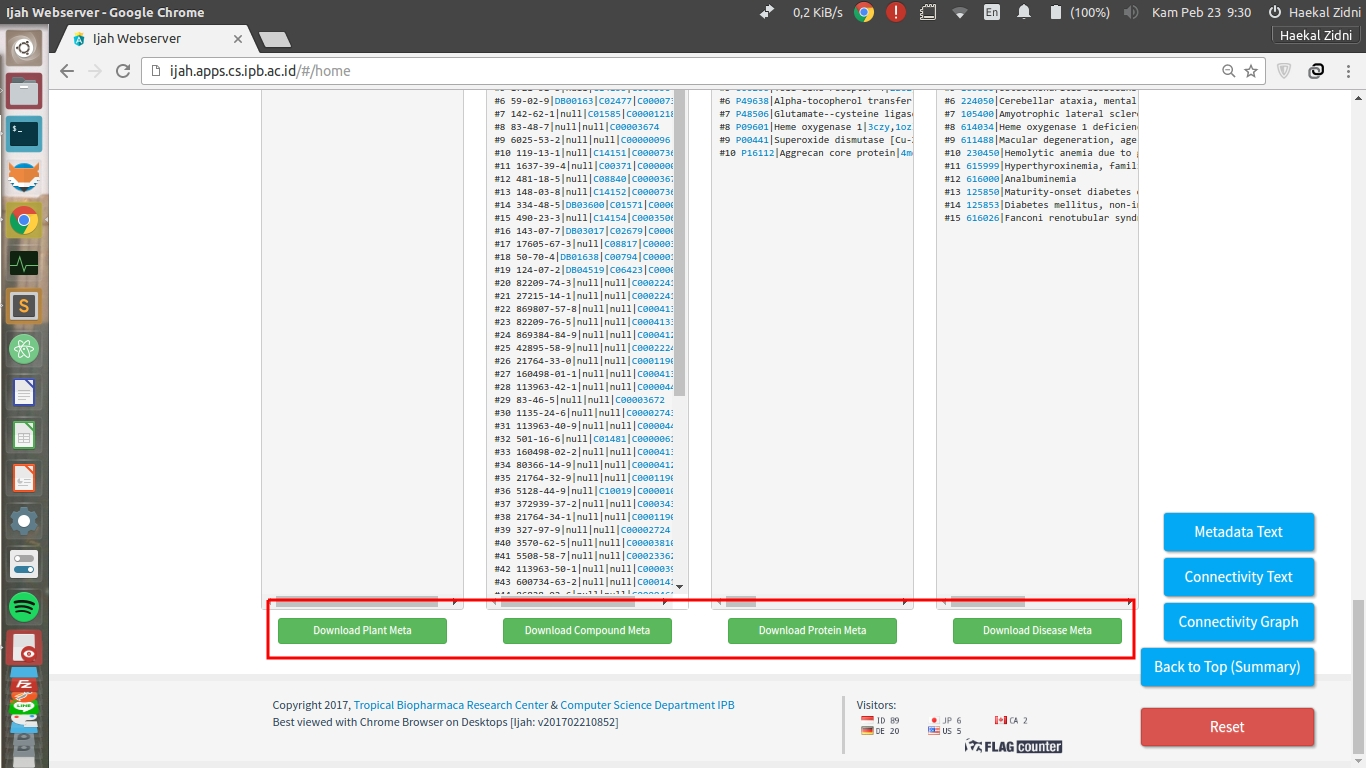
\includegraphics[scale=0.3]{ijah_meta_download.png}
% 	\caption{Tombol Download untuk mengunduh file \emph{Metadata Text Output}}
% 	\label{fig:ijah_meta_download}
% \end{figure}
